\documentclass[a4paper,11pt,fleqn,dvipsnames,twoside, openright ]{memoir} 	% Openright aabner kapitler paa hoejresider (openany begge)

%%%% PACKAGES %%%%

% ¤¤ Oversaettelse og tegnsaetning ¤¤ %
\usepackage[utf8]{inputenc}					% Input-indkodning af tegnsaet (UTF8)
\usepackage[english]{babel}					% Dokumentets sprog
\usepackage[T1]{fontenc}					% Output-indkodning af tegnsaet (T1)
\usepackage{ragged2e,anyfontsize}			% Justering af elementer
\usepackage{fixltx2e}						% Retter forskellige fejl i LaTeX-kernen
\usepackage{lscape}                         % For portræt mode i sideopsætning

% ¤¤ Figurer, tabeller (floats) og listings ¤¤ %
\usepackage{graphicx} 						% Haandtering af eksterne billeder (JPG, PNG, EPS, PDF)
\usepackage{epstopdf}
%\usepackage{eso-pic}						% Tilfoej billedekommandoer paa hver side
%\usepackage{wrapfig}						% Indsaettelse af figurer omsvoebt af tekst. \begin{wrapfigure}{Placering}{Stoerrelse}
\usepackage{multirow}                		% Fletning af raekker og kolonner (\multicolumn og \multirow)
\usepackage{multicol}         	        	% Muliggoer output i spalter
\usepackage{rotating}						% Rotation af tekst med \begin{sideways}...\end{sideways}
\usepackage{colortbl} 						% Farver i tabeller (fx \columncolor og \rowcolor)
\usepackage[table]{xcolor}					% Definer farver med \definecolor. Se mere: http://en.wikibooks.org/wiki/LaTeX/Colors
\definecolor{lightgray}{gray}{0.9}
\usepackage{flafter}						% Soerger for at floats ikke optraeder i teksten foer deres reference
\let\newfloat\relax 						% Justering mellem float-pakken og memoir
\usepackage{float}							% Muliggoer eksakt placering af floats, f.eks. \begin{figure}[H]
\usepackage{placeins}                       % \FloatBarrier
\usepackage{bytefield}                      %% Use for drwawing network packages
\usepackage{gensymb}
\usepackage{etex}                           % Er med for at få bytefields til at virke med hele gruppens LaTeX installationer.
\usepackage{listings}						% Placer kildekode i dokumentet med \begin{lstlisting}...\end{lstlisting}


% ¤¤ Matematik mm. ¤¤
\usepackage{amsmath,amssymb,stmaryrd} 		% Avancerede matematik-udvidelser
\usepackage{mathtools}						% Andre matematik- og tegnudvidelser
\usepackage{textcomp}                 		% Symbol-udvidelser (f.eks. promille-tegn med \textperthousand )
\usepackage{rsphrase}						% Kemi-pakke til RS-saetninger, f.eks. \rsphrase{R1}
\usepackage[version=3]{mhchem} 				% Kemi-pakke til flot og let notation af formler, f.eks. \ce{Fe2O3}
\usepackage{siunitx}						% Flot og konsistent praesentation af tal og enheder med \si{enhed} og \SI{tal}{enhed}
\sisetup{output-decimal-marker = {,}}		% Opsaetning af \SI (DE for komma som decimalseparator)

% ¤¤ Referencer og kilder ¤¤ %
\usepackage[english]{varioref}				% Muliggoer bl.a. krydshenvisninger med sidetal (\vref)
%\usepackage{natbib}							% Udvidelse med naturvidenskabelige citationsmodeller
\usepackage[style=numeric,natbib=true,backend=bibtex,bibencoding=ascii,sorting=none,maxnames=99,maxcitenames=1]{biblatex}
\usepackage{csquotes}
%\usepackage{xr}							% Referencer til eksternt dokument med \externaldocument{<NAVN>}

% ¤¤ Misc. ¤¤ %
\usepackage{lipsum}							% Dummy text \lipsum[..]
\usepackage[shortlabels]{enumitem}			% Muliggoer enkelt konfiguration af lister
\usepackage{pdfpages}						% Goer det muligt at inkludere pdf-dokumenter med kommandoen \includepdf[pages={x-y}]{fil.pdf}
\pdfoptionpdfminorversion=6					% Muliggoer inkludering af pdf dokumenter, af version 1.6 og hoejere
\pretolerance=2500 							% Justering af afstand mellem ord (hoejt tal, mindre orddeling og mere luft mellem ord)

% Kommentarer og rettelser med \fxnote. Med 'final' i stedet for 'draft' udloeser hver note en error i den faerdige rapport.
\usepackage[footnote,draft,english,silent,nomargin]{fixme}
%%%% CUSTOM SETTINGS %%%%

%%%% New Commands %%%%
\newcommand{\name}{Indoor positioning approch opens up new possiblities to childmolester and pedofiles in order to track the best children to target.}

% ¤¤ Marginer ¤¤ %
\setlrmarginsandblock{3.5cm}{2.5cm}{*}		% \setlrmarginsandblock{Indbinding}{Kant}{Ratio}
\setulmarginsandblock{2.5cm}{3.0cm}{*}		% \setulmarginsandblock{Top}{Bund}{Ratio}
\checkandfixthelayout 						% Oversaetter vaerdier til brug for andre pakker

%	¤¤ Afsnitsformatering ¤¤ %
\setlength{\parindent}{0mm}           		% Stoerrelse af indryk
\setlength{\parskip}{3mm}          			% Afstand mellem afsnit ved brug af double Enter
\linespread{1,1}							% Linie afstand

% ¤¤ Litteraturlisten ¤¤ %
%\bibpunct[,]{[}{]}{;}{a}{,}{,} 				% Definerer de 6 parametre ved Harvard henvisning (bl.a. parantestype og seperatortegn)
%\bibliographystyle{bibtex/harvard}			% Udseende af litteraturlisten.
%\bibliographystyle{unsrt}
\addbibresource{bib.bib}

% ¤¤ Indholdsfortegnelse ¤¤ %
\setsecnumdepth{subsection}		 			% Dybden af nummerede overkrifter (part/chapter/section/subsection)
\maxsecnumdepth{subsection}					% Dokumentklassens graense for nummereringsdybde
\settocdepth{subsection} 					% Dybden af indholdsfortegnelsen

% ¤¤ Lister ¤¤ %
\setlist{
  topsep=0pt,								% Vertikal afstand mellem tekst og listen
  itemsep=-1ex,								% Vertikal afstand mellem items
}

% ¤¤ Visuelle referencer ¤¤ %
\usepackage[colorlinks]{hyperref}			% Danner klikbare referencer (hyperlinks) i dokumentet.
\hypersetup{colorlinks = true,				% Opsaetning af farvede hyperlinks (interne links, citeringer og URL)
    linkcolor = black,
    citecolor = black,
    urlcolor = black
}

% ¤¤ Opsaetning af figur- og tabeltekst ¤¤ %
\captionnamefont{\small\bfseries\itshape}	% Opsaetning af tekstdelen ('Figur' eller 'Tabel')
\captiontitlefont{\small}					% Opsaetning af nummerering
\captiondelim{. }							% Seperator mellem nummerering og figurtekst
\hangcaption								% Venstrejusterer flere-liniers figurtekst under hinanden
\captionwidth{\linewidth}					% Bredden af figurteksten
\setlength{\belowcaptionskip}{0pt}			% Afstand under figurteksten


% ¤¤ Opsaetning af commands til semantic ¤¤ %
% Pil

\newcommand{\ra}[1][\relax]{\ensuremath \rightarrow_{#1}}
\newcommand{\Ra}[1][\relax]{\ensuremath \Rightarrow_{#1}}
\newcommand{\Raa}{\ensuremath \Rightarrow_{a}}
\newcommand{\Rab}{\ensuremath \Rightarrow_{b}}
\newcommand{\ram}{\ensuremath \rightarrow_{M}}
\newcommand{\Raexp}{\ensuremath \Rightarrow_{exp}}
\newcommand{\raexp}{\ensuremath \rightarrow_{exp}}
\newcommand{\RaS}{\ensuremath \Rightarrow_{S}}
\newcommand{\raS}{\ensuremath \rightarrow_{S}}
\newcommand{\rhu}{\ensuremath \rightharpoonup}
\newcommand\floor[1]{\lfloor#1\rfloor}
\newcommand\ceil[1]{\lceil#1\rceil}
% Logiske konnektiver

\newcommand{\logand}{\wedge}
\newcommand{\logor}{\vee}
\newcommand{\sand}{t\!\!t}
\newcommand{\falsk}{f\!\!f}

% Kantede parenteser

\newcommand{\lag}{\langle}
\newcommand{\rag}{\rangle}

% Next

\newcommand{\nexte}{\textrm{next}}

% Syntaks

\newcommand{\while}[2]{\texttt{while}\;#1 \; \texttt{do}\; #2}
\newcommand{\ifs}[3]{\texttt{if}\;\;#1 \; \texttt{then}\; #2 \; \texttt{else}\; #3}


% Regler

% Med sidebetingelse

\newcommand{\newcondinfrule}[3]
           {\parbox{5.5cm}{$$ {\frac{#1}{#2}}{\qquad
            #3} \hfill  $$}}

% Uden sidebetingelse

\newcommand{\infrule}[2]
           {\parbox{4.5cm}{$$ \frac{#1}{#2}\hspace{.5cm}$$}}

% Navne på regler

\newcommand{\runa}[1]{\mbox{\textsc{\protect{(#1})}}}
\newcommand{\runatt}[2]{$[{\mbox{\textsc{#1}}}_{\mbox{\textsc{\small #2}}}]$}

% Forkortelse for environments

\newcommand{\envv}{env_{v}}
\newcommand{\envp}{env_{P}}
\newcommand{\envm}{env_{m}}
\newcommand{\envf}{env_{f}}
\newcommand{\envs}{env_{s}}
\newcommand{\envi}{env_{i}}
\newcommand{\envvsf}{env_{vsf}}
\newcommand{\envl}{env_{l}}
\newcommand{\stoenvl}[2]{\ensuremath sto^{#1}, \envl^{#2}}
\newcommand{\ve}{\vdash_{E}}
\newcommand{\ev}{E \vdash}

% ¤¤ Opsaetning af listings ¤¤ %

\usepackage{mathdots} %Ensures that dots (especially the \vdots used in the lstlistings) are scaled along with the text size.
\newcommand{\csharp}{C\texttt{\#} } % C#
\newcommand{\codeDots}{\tiny{\raisebox{-2pt}[0pt][0pt]{$\vdots$}}} % Code dots


\definecolor{commentGreen}{RGB}{34,139,24}
\definecolor{stringPurple}{RGB}{208,76,239}

\lstdefinelanguage{inc_C}
{
	basicstyle=\small,
	basicstyle=\ttfamily\scriptsize,
	captionpos=b,
	showstringspaces=false,					% Mellemrum i strenge enten vist eller blanke
	numbers=left, numberstyle=\tiny,		% Linjenumre
	tabsize=4,
	frame=single,
	language=C
}

\lstdefinelanguage{inc_Java}
{
	basicstyle=\small,
	basicstyle=\ttfamily\scriptsize,
	captionpos=b,
	showstringspaces=false,					% Mellemrum i strenge enten vist eller blanke
	numbers=left, numberstyle=\tiny,		% Linjenumre
	tabsize=4,
	frame=single,
	language=Java
}

\lstdefinelanguage{our_bash}
{
	basicstyle=\small,
	basicstyle=\ttfamily\scriptsize,
        captionpos=b,
	showstringspaces=false,					% Mellemrum i strenge enten vist eller blanke
	numbers=left, numberstyle=\tiny,		% Linjenumre
	tabsize=4,
        frame=single,
        language=bash
}

\lstdefinelanguage{inc_cpp}
{
	basicstyle=\small,
	basicstyle=\ttfamily\scriptsize,
	captionpos=b,
	showstringspaces=false,					% Mellemrum i strenge enten vist eller blanke
	numbers=left, numberstyle=\tiny,		% Linjenumre
	tabsize=4,
	frame=single,
        keywordstyle=\color{blue}\ttfamily,
        stringstyle=\color{red}\ttfamily,
        commentstyle=\color{green}\ttfamily,
	language=C++
}



% ¤¤ Navngivning ¤¤ %
\addto\captionsenglish{
	\renewcommand\appendixname{Appendix}
	\renewcommand\contentsname{Table of Content}
	\renewcommand\appendixpagename{Appendix}
	\renewcommand\appendixtocname{Appendix}
	\renewcommand\cftchaptername{\chaptername~}				% Skriver "Kapitel" foran kapitlerne i indholdsfortegnelsen
	\renewcommand\cftappendixname{\appendixname~}			% Skriver "Appendiks" foran appendiks i indholdsfortegnelsen
}

% ¤¤ Kapiteludssende ¤¤ %
\definecolor{numbercolor}{gray}{0.7}		% Definerer en farve til brug til kapiteludseende
\newif\ifchapternonum

\makechapterstyle{jenor}{					% Definerer kapiteludseende frem til ...
  \renewcommand\beforechapskip{0pt}
  \renewcommand\printchaptername{}
  \renewcommand\printchapternum{}
  \renewcommand\printchapternonum{\chapternonumtrue}
  \renewcommand\chaptitlefont{\fontfamily{pbk}\fontseries{db}\fontshape{n}\fontsize{25}{35}\selectfont\raggedleft}
  \renewcommand\chapnumfont{\fontfamily{pbk}\fontseries{m}\fontshape{n}\fontsize{1in}{0in}\selectfont\color{numbercolor}}
  \renewcommand\printchaptertitle[1]{%
    \noindent
    \ifchapternonum
    \begin{tabularx}{\textwidth}{X}
    {\let\\\newline\chaptitlefont ##1\par}
    \end{tabularx}
    %\par\vskip-2.5mm\hrule
    \else
    \begin{tabularx}{\textwidth}{Xl}
    {\parbox[b]{\linewidth}{\chaptitlefont ##1}} & \raisebox{-15pt}{\chapnumfont \thechapter}
    \end{tabularx}
    %\par\vskip2mm\hrule
    \fi
  }
}											% ... her

\chapterstyle{jenor}						% Valg af kapiteludseende - Google 'memoir chapter styles' for alternativer

% ¤¤ Sidehoved ¤¤ %

\makepagestyle{AAU}							% Definerer sidehoved og sidefod udseende frem til ...
\makepsmarks{AAU}{%
	\createmark{chapter}{left}{shownumber}{}{. \ }
	\createmark{section}{right}{shownumber}{}{. \ }
	\createplainmark{toc}{both}{\contentsname}
	\createplainmark{lof}{both}{\listfigurename}
	\createplainmark{lot}{both}{\listtablename}
	\createplainmark{bib}{both}{\bibname}
	\createplainmark{index}{both}{\indexname}
}
\nouppercaseheads											% Ingen Caps oenskes

\makeevenhead{AAU}{sw403f15}{}{\leftmark}				% Definerer lige siders sidehoved (\makeevenhead{Navn}{Venstre}{Center}{Hoejre})
\makeoddhead{AAU}{\rightmark}{}{Aalborg University}		% Definerer ulige siders sidehoved (\makeoddhead{Navn}{Venstre}{Center}{Hoejre})
\makeevenfoot{AAU}{\thepage}{}{}							% Definerer lige siders sidefod (\makeevenfoot{Navn}{Venstre}{Center}{Hoejre})
\makeoddfoot{AAU}{}{}{\thepage}								% Definerer ulige siders sidefod (\makeoddfoot{Navn}{Venstre}{Center}{Hoejre})
\makeheadrule{AAU}{\textwidth}{0.5pt}						% Tilfoejer en streg under sidehovedets indhold
\makefootrule{AAU}{\textwidth}{0.5pt}{1mm}					% Tilfoejer en streg under sidefodens indhold

\copypagestyle{AAUchap}{AAU}								% Sidehoved for kapitelsider defineres som standardsider, men med blank sidehoved
\makeoddhead{AAUchap}{}{}{}
\makeevenhead{AAUchap}{}{}{}
\makeheadrule{AAUchap}{\textwidth}{0pt}
\aliaspagestyle{chapter}{AAUchap}							% Den ny style vaelges til at gaelde for chapters
															% ... her

\pagestyle{AAU}												% Valg af sidehoved og sidefod


%%%% CUSTOM COMMANDS %%%%

% ¤¤ Billede hack ¤¤ %
\newcommand{\figur}[5]{
		\begin{figure}[#1] \centering
			\includegraphics[width=#2\textwidth]{graphics/#3}
			\caption{#4}\label{#5}
		\end{figure}
}

%%%% SIGNATUR %%%%%
\newcommand{\signature}[1]{
\begin{minipage}[c]{\textwidth}
\vspace{2cm}

\makebox[7cm][c]{
\hfill \makebox[7cm] {\hrulefill}
}

\makebox[7cm][c]{
 \hfill #1 \hfill
}
\end{minipage}
}

%%%% Personlige FixMes %%%%
\newcommand{\ofx}[1]{
\fxnote{Oliver: #1}
}
\newcommand{\jfx}[1]{
\fxnote{Jacob: #1}
}
\newcommand{\afx}[1]{
\fxnote{Anders: #1}
}
\newcommand{\sfx}[1]{
\fxnote{Simon: #1}
}

% ¤¤ Specielle tegn ¤¤ %
\newcommand{\decC}{^{\circ}\text{C}}
\newcommand{\dec}{^{\circ}}
\newcommand{\m}{\cdot}

\usepackage[noabbrev]{cleveref}						% Tillader brug af \cref, skal stå efter hyperref for at virke

%%%% ORDDELING %%%%

\hyphenation{}
\raggedbottom
\begin{document}
%%% file for glossaries
%\newglossaryentry{label}
%{
%  name={name},
%  description={text}
%}
%%%%%
%\newacronym{label}{short}{long}
%%Nedenstående er til flertal hvor der ikke bare skal s på enden
%\newacronym[longplural={Frames per Second}]{fpsLabel}{FPS}{Frame per Second}
%%
%%eksempler_start%%
   %\newacronym{pthread}{Pthreads}{POSIX threads}

   %\newglossaryentry{nix}
   %{
   %  name={*NIX},
   %  description={*NIX is a general term for Unix and Unix Like systems (e.g Linux, BSD and Mac OS X)}
   %}
%%eksempler_slut%%
\frontmatter													% Forindhold - nummereres med romertal
\thispagestyle{empty}
\begin{flushright}
\vspace{3cm}

\phantom{hul}

\phantom{hul}

\phantom{hul}

\textsl{\Huge \name{}} \\ \vspace{1cm}

\rule{13cm}{3mm} \\ %\vspace{1.5cm}
%\vspace{1cm}
\end{flushright}

\begin{center}
%\includegraphics[scale=0.30]{billeder/yggdrasil.jpg}
%\\\textcolor{gray}{Yggdrasil -By Leliumoj \cite{asgard_img}}
\end{center}
\begin{flushright}
\vspace{2cm}
\textsc{\Large P6 Project \\
Group SW608F16 \\
Software\\
Aalborg University\\
26\textsuperscript{th} May 2016\\

\includegraphics[width=0.25\textwidth]{graphics/AAU-logo-stud-UK-RGB.pdf}}
\end{flushright}
\cleardoublepage												% Indsaetter tom side, saa naeste kapitel starter paa hoejre side (hvis noedvendigt)
% Dette er LaTeX-versionen af titelbladet for TNB studenterrapporter
% Filen kræver:
% Universitetets logo:  AAU-logo-stud-UK eller AAU-logo-stud-DK
% Synopsis: En fil ved navn synopsis.tex

% Udarbejdet af: Jesper Nørgaard (jesper@noergaard.eu) 10. april 2012

\phantomsection
\pdfbookmark[0]{Title page}{Title page}
\thispagestyle{empty}

\begin{minipage}[t]{0.48\textwidth}
\vspace*{-25pt}			%\vspace*{-9pt}

\includegraphics[height=4cm]{graphics/AAU-logo-stud-UK-RGB.pdf}
\end{minipage}
\hfill
\begin{minipage}[t]{0.48\textwidth}
{\small
\textbf{Department of Computer Science}\\
Software \\
Selma Lagerlöfs Vej 300 \\
9220 Aalborg East \\
https://www.cs.aau.dk}
\end{minipage}

\vspace*{1cm}

\begin{minipage}[t]{0.48\textwidth}
\textbf{Title:} \\[5pt]\bigskip\hspace{2ex}    
(S)PiCams\\
\textbf{Project:} \\[5pt]\bigskip\hspace{2ex}
P5

\textbf{Project period:} \\[5pt]\bigskip\hspace{2ex}
September 2015 - December 2015

\textbf{Project group:} \\[5pt]\bigskip\hspace{2ex}
SW508E15

\textbf{Members:} \\[5pt]\hspace*{2ex}
Martin Kristjansen \\\hspace*{2ex}
Jonas S. Madsen \\\hspace*{2ex}
Anders L. Matthiassen \\\hspace*{2ex}
Lars Nielsen \\\hspace*{2ex}
Simon A. Pedersen \\\hspace*{2ex}
Christian Stephansen


\textbf{Supervisor:} \\[5pt]\hspace*{2ex}
Johannes Lindhart Borresen


\vspace*{1cm}

\textbf{Prints: 8} \\
\textbf{Pages: 99} \\
\textbf{Appendices: 2} \\
\textbf{Ended: 21-12-2015}

\end{minipage}
\hfill
\begin{minipage}[t]{0.483\textwidth}
Synopsis: \\[5pt]
\fbox{\parbox{7cm}{\bigskipThis report covers the subjects of designing an embedded system for target tracking in a 3D space. The focus is to design a surveillance system, which is achieved through the use of multiple camera units performing object recognition. Furthermore, the system has extended functionality which allows for target tracking, by using a laser pointer mounted on a Lego-constructed rig controlled by two dc motors.

The general flow of information in the system is as follows: the camera units, composed of Raspberry Pis and webcams, each obtain information about a recognised object and calculate the object's direction relative to the camera. This information is communicated through a modem to an NXT brick, where a triangulation is performed to determine where the object is relative to the Lego-constructed rig. 

The system's dependability is analysed which presents the relevant attributes in the designed system. The relevant actuator tests of the designed system is presented and the results are analysed. The theory behind object recognition is introduced and explained.\bigskip}}
\end{minipage}

\vfill

{\footnotesize\itshape The content of the report is freely available, but publication (with source reference) may only take place in agreement with the authors.}

% Rapportens indhold er frit tilgængeligt, men offentliggørelse (med kildeangivelse) må kun ske efter aftale med forfatterne.
% The content of the report is freely available, but publication (with source reference) may only take place in agreement with the authors.

\cleardoublepage
\chapter*{Preface}

\textbf{Reading guidance}\\


In the report source references are presented by a version of the Vancouver system, where sources are indicated by square brackets. An example is [1], where this is the first source in the bibliography.


\begin{multicols}{2}
\signature{Oliver B. Købsted}
\signature{Anders L. Matthiassen}
\signature{Jacob Nielsen}
\signature{Simon A. Pedersen}
\end{multicols}
\cleardoublepage

\phantomsection													% Kunstigt afsnit, som hyperlinks kan 'holde fast i'
\pdfbookmark[0]{Table of Contents}{Contents}					% Tildeler en klikbar bookmark til den endelige PDF
\tableofcontents*												% Indholdsfortegnelsen (kaldet ToC)

%\addtocontents{toc}{\protect\newpage}							% Fremtvinger sideskift i ToC hvis noedvendig (der hvor koden placeres)

\mainmatter	\setcounter{page}{1}													% Hovedindhold - nummereres fra side 1


%%Indsæt rapportens filer her!!%%
\chapter{Introduction}\label{chpt:introduction}
Surveillance is becoming an increasingly more important aspect in present day. In an attempt to increase the safety of its citizens, governments all over the world install public cameras\cite{city_surveillance}. At the same time the dream of intelligent robots with human-like behaviour, as depicted in movies such as "I, Robot"\cite{imdb_robot}, is nearing. Development of artificial intelligence is a hot topic in 2015, and several experts predict that  soon will be an integral element of everyday life\cite{ai_microsoft}.

An important element of programming machines to exercise human-like behaviour is the ability to sense and interact with their environment. Giving a machine senses is one thing, but teaching the machine how to react on these sensing inputs is an extremely complex task\cite{facebook_ai}. A problem as simple as using a camera to simulate vision and then finding and recognising a complex object, such as the face of a person, is a computationally heavy task\cite{ai_facial_recog}.

%Recognition can also be used in a militaristic context. A system could be able to recognise objects, say an enemy vehicle, and follow this vehicle's movement, waiting for permission to fire\cite{rockwell_system}. Soldiers in the field could then carry a device that they could quickly be set up and use for monitoring an area, perhaps even with several cameras to have a greater  to monitor. Another system could be set up to monitor and protect embassies in foreign countries by tracking and shooting unrecognised intruders.

%værdifulde genstande
Recognition is also used for security systems in buildings with valuable possessions. Such a location could be a museum with irreplaceable objects like paintings and other artefacts, which need to be kept safe from intruders. The challenges this system could face are tasks such as monitoring a 3D space, identifying and distinguishing valuable artefacts from objects of no interest and continue tracking them in motion.

This project aims to build a simplified version of the museum security system and explores the theme of surveillance, in connection with embedded devices, with the primary focus of creating a targeting platform that is able to recognise a predefined object. The system will incorporate a secondary focus of tracking the object with the intention of notifying some second system to ensure the safety of the predefined object.

\chapter{Context and Requirements}\label{chpt:context_spec}
In order to provide a solution for the problem, a set of requirements must be defined for the context. However, before the requirements engineering, an overall setup has to be specified, since this has an influence on how the requirements are defined and prioritised. 

\section{Problem and System Setup}\label{sec:base_setup}
The simplified problem is that a surveillance system as a primary function must be able to recognise and monitor an object by the use of multiple cameras, secondarily the system should track the object and notify some secondary system of any present intruder.

Cameras capture 2D images and with the use of several cameras, with overlapping \gls{fov}, it is possible to calculate an object's position in 3D space, once the object is in one of the overlapping \glspl{fov}. When an object has been recognised by the system, the secondary focus comes in effect and tracks the object. It is possible to track an object in several ways. For this project the tracking unit is chosen to be a laser pointer which will aim at the object. This gives an easy way of getting immediate feedback by physically visualising what the system recognises. An important aspect of this feedback is that it can be used to easily compare the system's internal representation with the object's actual position. 

The tracking of a recognised object may fail without consequences for the primary functionality, as the system can always fall back to monitoring. The second system will not be developed as part of this project, but will be notified of the intruder's position trough tracking of the predefined object.

The basic setup consists of two types of devices: static camera units and a tracking unit. The tracking unit is able to rotate in order to follow a recognised object. The setup might be expanded in order to fulfil the requirements. With the basic setup defined, the requirements can now be specified. 
\section{Requirements}\label{sec:requirements}
\Cref{tbl:requirement} lists the requirements in prioritised groupings, with the most essential requirement as \textit{Must have}. The requirements will be specified in the following.

\begin{table}[h]
    \centering
    \begin{tabular}{|c|}
    \hline
     \textbf{Must have} \\ \hline
     Object Recognition \\ \hline
     Target Tracking \\ \hline\hline
     \textbf{Good to have} \\ \hline
     Advanced Object Recognition \\ \hline
     Advanced Target Tracking \\ \hline
     Advanced Target Acquisition\\ \hline\hline
     \textbf{Stretch Goal} \\ \hline
     Turning Cameras \\ \hline 
    \end{tabular}
    \caption{Requirement table}
    \label{tbl:requirement}
\end{table}

The requirements have been chosen and prioritised doing a brainstorm session, based on the context described earlier and represents different features that will support the problem definition.

\emph{Object Recognition}\\
Means to recognise a predetermined object in a image, and to determine the position in said image. 

\emph{Target Tracking}\\
When a camera has recognised the predefined object, the specific position of the object, in respect to the camera, is calculated. When the pointing device has information from multiple cameras, the position of the object, in regards to the pointing device, is calculate and the pointing device is instructed to move the pointer in the direction of the object.

\emph{Advanced Object Recognition}\\
This requirement specifies the attribute of recognising different objects in a single image from one camera.

\emph{Advanced Target Tracking}\\
If the system recognises multiple objects simultaneously, the system must be able to utilise the same amount of pointing devices, such that all objects are tracked.

\emph{Advanced target Acquisition}\\
The system can use more than two cameras in order to acquire a target. The use of multiple cameras allows the system to cover rooms larger than what is possible with two cameras. The accuracy of the pointing device can be improved as the position is based on multiple sources and thereby it is possible to discard positions that, according to the system, stands out.


\emph{Turning Cameras}\\
By expanding the system to include cameras that are able to turn, the amount of cameras needed to cover a room is decreased because each camera is able to cover a bigger area.
\section{Coordinates Specification}\label{sec:coor}
In order to design the software used to calculate an object's position in 3D space, a global coordinate system must be defined. In \ref{sec:base_setup} it is described that there is a single laser unit and two or more camera units. All the camera units must have a position and direction in the global coordinate system, if an object's position is to be calculated. The laser unit's position and direction relative to the object must also be known for it to point towards the object.

The origin of the system is defined be at the pointing device. Choosing the laser unit as the origin, its position becomes unambiguous. In order to implement this, a specific point of the pointing device must be chosen. 

To use a global coordinate system, the pointing device and camera units must have a procedure for calibration. This calibration ensures that the initial directions of the laser and views are known, which in turn makes it possible to calculate the object's position and have the laser unit point towards it. 
\chapter{Hardware Selection}
\label{chp:tech}
In this chapter a description of both the hardware and software components utilised in the system setup will be presented. These components are designed and developed by external suppliers, and the description will contain the argumentation for why it has been chosen to utilise a given component.

The descriptions include how hardware is used for the laser unit and camera units, how these units interact and how the final system setup is structured as a result of the choices.

\section{Laser Unit}\label{sec:laser}
The base setup in \cref{sec:base_setup} describes how a laser unit must point towards a target if this target is identified by the camera units. This section described the hardware used for this task and the operating system used for the hardware. 
\subsection{\acrlong{nxt}}\label{ss:nxt}
The \gls{nxt} is a part of the Lego Mindstorms series which offers the possibility to create small robots using the components provided with a Lego Mindstorms NXT 2.0 set\cite{lego_mindstorms}.  This set includes a set of different sensors, actuators and a \gls{nxt} intelligent brick. The \gls{nxt} is a embedded device that can communicate the actuators and sensors included in the \gls{nxt} set. It is also possible for the \gls{nxt} to communicate with other devices with over wired and wireless connections. Some of its hardware specifications are presented in \cref{tbl:nxt_spec}, where it communication protocols also are listed.

\begin{table}[ht]
  \centering
  \begin{tabular}{|l|r|}
  \hline
    Main microcontroller & 32-bit Atmel AT91SAM7S256, 256KB Flash memory, 64 KB RAM \\ \hline
    Microcontroller & 8-Bit Atmel ATmeg48, 4 KB flash memory, 512 Bytes RAM \\ \hline
    Bluetooth  & CSR BlueCore\textsuperscript{TM} 4 v2.0 +EDR System \\ \hline
    Wired communication  & RS485, I\textsuperscript{2}C and USB\\ \hline
    Input ports & Four 6-pin input ports numbered 1 to 4 \\ \hline
    Output ports & Three 6-pin outputs ports denoted A to C\\  \hline
  \end{tabular}
  \caption{\gls{nxt} Intelligent brick specification\cite{lego_hardware}}
  \label{tbl:nxt_spec}
\end{table}

One actuator of the \gls{nxt} set is DC motors\cite{lego_mindstorms}, which can be used when designing a target tracking system. The motors can be used for creating the mechanism for pointing to a given target as described in the requirements in \cref{chpt:context_spec}. Each motor has a internal tick counter which have a resolution on one degree, which means that the motors has moved 360 ticks for each turn around\cite{nxt_motor}. The motors are controlled by sending instructions from the \gls{nxt} intelligent brick.

The \gls{nxt} and motors can be used in conjunction with the normal Lego bricks which offers the possibility to easily modify the construction of the laser unit. Since it can easily be modified it offers a good opportunity to experiment on the setup which is an advantages. Both the motors and \gls{nxt} intelligent brick can be used as components which makes it possible to do target tracking. Considering this it has been decided to use the \gls{nxt} set as a part of the laser unit in the hardware solution.

\subsection{nxtOSEK}
The \gls{nxt} comes with a \gls{os} written by the Lego Corporation. It could be beneficial to change the firmware of the \gls{nxt} in order to more control. An example is have more control of how resources are managed.

In order to get this control of the \gls{nxt}, the nxtOSEK \gls{os} is used as it can used to utilise the processors, schedule tasks and so forth. This \gls{os} is a \gls{rtos} so it is also suitable for fulfilling the real-time requirements. Furthermore, nxtOSEK supports floating-point precision, which will be needed in the calculations for targeting an object. NxtOSEK provides a C and C$++$ API for sensors and actuators that can be used with the \gls{nxt}.

Given that nxtOSEK is a \gls{rtos} relevant real time requirements for target tracking. If the purpose of the system is only to track a target there might be soft real time requirements. The reason for them to be soft is that the system does not fail if a single set of data from the sensors is not handled at the deadline. If several deadlines are missed it could potentially result in loosing track of target. Using a \gls{rtos} it is possible to determine whether or not tracking a target is possible with the designed system.
\section{Camera Units}
\label{s:cu}
In \cref{sec:base_setup} the base setup describes the principle of using several camera units in order to make a laser unit point towards a target. This section described the hardware chosen for this task and what it fulfil the needs for the system setup.
\subsection{Camera Type}
\label{ss:cam_type}
If an object is to be tracked by a laser, the position of the object has to be obtained by camera units as described in \cref{sec:base_setup}. This section presents two different types of cameras that could be used in this project and the pros and cons of each possibility.

One possible camera that can be used for the system is the Microsoft Kinect. This camera also provides other features, some of which could be useful for the project, such as built-in body motion tracking, depth sensors and night vision\cite{kinect}. The motion tracking and depth sensors can be used to obtain the intruders position and the dark vision makes it possible to track objects regardless of the light intensity. One issue of the Kinect is the retail price as it costs 1199 DKK\cite{kinect_price}. To have full coverage of a room it can be necessary to use several Kinects. This is because the room could be too big or that there are objects, such as furniture, which results in blind spots for the Kinect. The effect of using the Kinect is therefore an increase in cost for the system in exchange of having the additional functionality of the Kinect.

\begin{figure}[ht]
  \centering
  \includegraphics[scale=0.1]{graphics/cvbw3.jpg}
  \caption{\gls{cvbw3} chosen for the project.}
  \label{fig:cvbw3}
\end{figure}

An alternative solution is having webcams with no functionality aside from providing a stream of 2D images. The stream of images can be used to get the direction of the object relative to the respective webcam. To achieve a similar functionality as the first solution with respect to the ability of calculating the depth of an object, it will be necessary to use more than one webcam to triangulate an objects position. An example of a webcam that provides this functionality is the \acrfull{cvbw3}\cite{video_blaster}, which is illustrated in \cref{fig:cvbw3}, but any webcam with the functionality of providing a stream of 2D images will do. The major advantage of this solution is the price; a cheap consumer webcam bought at a Danish retailer is estimated to be around 150 DKK, as seen on price comparison sites\cite{pricerunner_webcam}\cite{ebd_webcam}.

The project has been offered six \acrfull{cvbw3}\cite{video_blaster}, which afford the required functionality while also being relatively old, as they are produced in 1999. In this sense the project also serves to show the possibility of using newer webcams that are equally or more sophisticated in terms of point of view and resolution. This offer was accepted since the cameras have the desired functionality. A consequence of this choice is that the \gls{cvbw3} communicates over USB, which limits what devices that can be used to analyse the image stream.
\subsection{Transfer Device}
\label{sec:rsp}
In order to collect data from a camera, prepare data for transfer and sending data to the \gls{nxt}, a device is needed to handle the communication and data manipulation.
There exists multiple devices which allow for the possibility of connecting to a camera along with manipulating and sending the data to the \gls{nxt}. The project has a focus on embedded devices, amongst these devices is the \gls{Arduino} board and the Raspberry Pi.

The \gls{Arduino} is an open source microcontroller based circuit board, for building digital devices \cite{ard_1}. The Arduino comes with the possibility of extending the capabilities of the board by additional hardware components. To enable communication with a camera over a USB connection, a USB shield is needed. The \gls{Arduino}'s extensibility also allow for network communication using an ethernet shield, such as the \gls{Arduino} Ethernet Shield 2 \cite{eth_shl_1}. An \gls{Arduino} UNO with shields for ethernet connection and USB communication costs approximately 635 DKK in retail price, not including shipping.

The Raspberry Pi is a single-board computer \cite{rsp} and is commonly used for educational purposes and embedded systems, running with a Linux based operating system. The Raspberry Pi comes with built-in USB and ethernet capabilities, which can be used for communication with both a camera and a \gls{nxt}. As the Raspberry Pi already contains the required hardware there is no need to buy additional hardware components, as opposed to the \gls{Arduino} board. However, it is necessary to buy a power adapter and as such the total cost of a Raspberry Pi is approximately 291 DKK in retail price, not including shipping \cite{rs_pi_board}\cite{rs_chg}.

The Raspberry Pi is less expensive than the \gls{Arduino} board, and is also an all-in-one solution, as such it has been chosen as the hardware component for the project. Choosing the Raspberry Pi has the extra benefit of it being significantly more computationally powerful than the standard \gls{Arduino} board, which gives more freedom when designing the system.

\begin{table}[ht]
  \centering
  \begin{tabular}{|l|r|}
  \hline
    System On a Chip & Broadcom BCM2835 \\ \hline
    CPU & 700 MHz single-core ARM1176JZF-S \\ \hline
    GPU & Broadcom VideoCore IV @ 250 MHz \\ \hline
    Memory & 512Mb SDRAM, shared with GPU \\ \hline
    Storage & None - option of connecting SD Card \\ \hline
    Network & 10/100 MBit/s Ethernet \\ \hline
    USB & 2 USB 2.0 Ports \\    \hline
  \end{tabular}
  \caption{\gls{rsp} Model B specification\cite{rsp2}}
  \label{tbl:rsp_spec}
\end{table}

\section{Inter-device Communication}
In the previous sections the \gls{nxt} and \gls{rsp} were chosen as the hardware for communicating between the laser unit and camera units. This system will consist of a single \gls{nxt} and several \glspl{rsp}; one for each \gls{cvbw3}. The \gls{nxt} needs to get information from every camera that is able to see the target in order to point its laser towards it. This section evaluates the options for communication between the camera units and the laser unit.

In order to minimize delay and uncertainties it has been chosen to use a wired connection, which excludes a Bluetooth connection. The available alternatives for wired communication for the \gls{nxt} are the RS485, I\textsuperscript{2}C, and USB protocols\cite{lego_hardware}.

The RS485 protocol is only supported by the \gls{rsp} if an extra shield is used\cite{rs485_shield}. This makes it a less preferable solution as additional shields are needed for every \gls{rsp}.

The I\textsuperscript{2}C protocol is a master-slave protocol that can be used both by the \gls{rsp} and by the \gls{nxt}. However, neither of the two devices can be slave. The \gls{nxt} does outright not have the option of being slave\cite{lego_hardware} and if the \gls{rsp} is to be slave, two GPIO pins are needed; one for the data transfer and one for clock reference. The pin for the clock is not connected on Model B\cite{pi_gpio_1}\cite{pi_gpio_2} so this protocol is not an option since the \gls{rsp} Model B is used for this project.

The last option is a USB connection as both the \glspl{rsp} and the \gls{nxt} have USB-ports. Lego has released a Windows driver for the \gls{nxt}\cite{lego_driver}. However, with only 512mb of flash memory it has been chosen not to install a Windows OS on the \glspl{rsp} and therefore it is not a solution to directly connectet a \gls{rsp} with a \gls{nxt} by USB.  

None of the three options can be used to directly connect the \gls{nxt} to the \glspl{rsp}. The I\textsuperscript{2}C protocol can not be used with the chosen hardware while the two other options needs additional hardware. Since no protocol is supported by both the \glspl{rsp} and the \gls{nxt}, an intermediate component must be integrated. One possibility is to have a laptop to act as a modem between the \glspl{rsp} and the \gls{nxt}. Acquiring a laptop, Ethernet cables and a switch is considered to be easier than ordering RS485 shields for the \glspl{rsp} which made it an easy solution for the inter-device communication. If the computer is connected to a switch with Ethernet, all \glspl{rsp} can connect to the same switch through Ethernet cables, and as such the devices can communicate. The laptop will be running Windows since it can use the released USB driver and thereby connect to the \gls{nxt}. 
\section{System Design}
\label{sec:system_design}
The \glspl{rsp} model B and \gls{nxt} has been chosen as the hardware to control the laser unit and camera units. For these units to be able to communicate, an intermediate device is integrated in the system. This device is a laptop running a Windows OS which uses USB to communicate with the \gls{nxt} and Ethernet to communicate with the \glspl{rsp}. This section explores the possibilities for the dataflow and at which points calculations can be performed in order to provide a solution for the problem presented in \cref{sec:base_setup}.

It has been chosen to keep all calculations outside of the computers scope. This decision has been made because the computer is intended as a means of communication. By simply letting it be a modem, one could in theory use any device capable of running a Windows OS, and using the USB driver, for the task of communicating data. This intermediate device can be chosen regardless of its computational capabilities as no computational power is needed.

There are two key calculations that have to be performed in the system. Firstly, every image captured with the \glspl{rsp} have to be analysed, and secondly, the results have to be gathered and used for calculating where the laser has to point to. It is obvious that these two calculations have to be done in sequence; it does not make sense to attempt calculating where the laser has to point without having something to point at. It was discovered in \cref{sec:rsp} that the \gls{rsp} is computationally powerful, and comparing the specifications of the \gls{rsp} with the \gls{nxt}, as seen in \cref{tbl:rsp_spec} and \cref{tbl:nxt_spec}, reveals that the \gls{rsp} is significantly more powerful than the counterpart. It is therefore more fit for the task of analysing images than the \gls{nxt}. Performing this calculation on the \glspl{rsp} also means less data have to be transferred, as the size of the image analysis result is smaller than the size of the image. The \gls{nxt} can then collect the data and calculate where it needs to point to.

Alternatively the \gls{nxt} can perform both calculations. However, doing this results in more data being communicated between the devices, as every \gls{rsp} in the system has to transfer an image to the \gls{nxt}, and ultimately there is a risk that the microcontroller on the \gls{nxt} is too slow at performing the tasks and performance will be degraded. The amount of data transferred increases significantly as more camera units are integrated in the system. This increase is much smaller if the first task is performed immediately on the \glspl{rsp}.

On the basis of the limitations of the \gls{nxt}, and the amount of data that needs to be communicated, it has been decided to use the \gls{rsp} for performing the image analysis. The results are then transferred to the \gls{nxt}, which uses these results to calculate where it has to point at.

\chapter{Rig Construction}\label{sc:rig}
Based on the system requirements specified in \cref{sec:requirements} and the hardware components presented in \cref{chp:tech}, there have been construct two setup design ideas for constructing a rig, which will comply to the requirements and use the selected hardware components.

Both setup design ideas are designed to track a object in a 3D space for this two things components are used, firstly a laser pointer to mark the target and secondly the component for moving the laser point in a 3D space, this component is the DC motor which are include in the \acrfull{nxt} set. It has been selected to use one motor for horizontal movement and one for vertical movement.


To use the \gls{nxt} motors for moving a pointer, a rig is constructed with Lego bricks. This section presents two ideas to construct the rig and decides upon the presented setups. When evaluating the two setups it is important to assess the impact on factors such as stability of the rig, rotational freedom and the centres of the horizontal and vertical rotation axes.

\section{First Setup}\label{sec:first_setup}
The first setup, as seen on \cref{fig:rig_flat}, has a gear directly on a motor used for rotation of the vertical axis, illustrated on \cref{fig:rotation_defs}. The gear connected to the motor has a 90\degree\ connection to another gear which is part of a rotational turret, a close-up of this is shown on \cref{fig:rig_horizontal_base}. The other motor for rotation of the horizontal axis is fixated on the rotational turret. The motor has multiple fix points which is greatly beneficial for the stability.

A complication that arise from the setup is the need to define an offset, as the origin of the global coordinate system has its base in the intersection of the two axes. The offset is the distance between the base point to the vertical axis, which is the motor that has the laser attached to it. The offset is used when a rotation in the vertical plane is performed as the base point for the horizontal axis rotation is moved in the global coordinate system, and a calculation of the new position must be executed. Regarding the rotational freedom, the vertical rotation motor can move freely, when not considering the other motor. Restrictions for the rotations are that a cable must be connected to the motor for the horizontal rotation, which restricts the otherwise freely moving vertical motor. Furthermore the pointing device that must be connected to the horizontal motor, restricting the pointer in being able to do a 360\degree\ rotation. A close-up of the setup for the pointer is seen on \cref{fig:rig_horizontal_rotation}.
\begin{figure}[H]
	\begin{minipage}{0.5\textwidth}
		\centering
    	\includegraphics[width=0.80\textwidth]{graphics/rotation_definitions.jpg}
    	\caption{Illustrations of rotational axes \cite{rotation_definitions}}
    	\label{fig:rotation_defs}
	\end{minipage}
	\begin{minipage}{0.5\textwidth}
		\centering
    	\includegraphics[width=0.80\textwidth]{graphics/rig/rig_flat_entire.jpg}
    	\caption{First setup}
	    \label{fig:rig_flat}
	\end{minipage}
\end{figure}

\begin{figure}[H]
    \begin{minipage}{0.5\textwidth}
    	\centering
    	\includegraphics[width=0.80\textwidth]{graphics/rig/rig_horizontal_turret.jpg}
    	\caption{close-up of rotational turret for first setup}
    	\label{fig:rig_horizontal_base}
    \end{minipage}%
	\begin{minipage}{0.5\textwidth}
    	\centering
    	\includegraphics[width=0.80\textwidth]{graphics/rig/rig_vertical.jpg}
    	\caption{close-up of setup for rotation of horizontal axis}
    	\label{fig:rig_horizontal_rotation}
	\end{minipage}
\end{figure}

\section{Second Setup}
The second setup utilizes the same base structure for the rotation of the vertical axes with the 90\degree\ connected gears. But the Lego turret brick is of another model which results in the motor for horizontal rotation to be placed upright. A gain from this setup is that the rotational bases are placed directly on top of each other making the definitions thereof more simple than the first setup, as the base point of the horizontal rotational axis does not require recalculation. However, the upright placement of the motor results in fewer fix points and a more unstable connection, having the pointer vibrate greatly when either motor is moved. Another version of the setup gave better stability but resulted in the upright motor base point to be pushed off-centre. Pictures of both versions are shown in \cref{fig:rig_unstable} and \cref{fig:rig_stable}. Lastly the rotational freedom for the second setup is the same as for the first setup where the pointer is connected to the horizontal rotation axis, and a cable is connected to the motor, which restricts the rotation of the vertical rotational axis.

\begin{figure}[H]
    \centering
    \includegraphics[width=0.50\textwidth]{graphics/rig/rig_standing_entire.jpg}
    \caption{Second setup}
    \label{fig:rig_standing}
\end{figure}

\begin{figure}[H]
    \begin{minipage}{0.5\textwidth}
	\centering
	    \includegraphics[width=0.80\textwidth]{graphics/rig/rig_standing_unstable.jpg}
	    \caption{Close-up of unstable setup}
	    \label{fig:rig_unstable}
    \end{minipage}%
	\begin{minipage}{0.5\textwidth}
		\centering
	    \includegraphics[width=0.80\textwidth]{graphics/rig/rig_standing_stable.jpg}
	    \caption{Close-up of stable setup}
	    \label{fig:rig_stable}
	\end{minipage}
\end{figure}

\section{Final Setup}
The elected setup is the first setup mainly because of its stability. Both setups have the same rotational freedom, therefore it is not taken into consideration. Considering the base points, the vertical base point will be the same, but looking at the horizontal the unstable version of the second setup has great benefits for calculating the base point. However, the instability is to much of a disadvantage. This could be solved for the setup by stabilising it, but that leaves it with the same disadvantages regarding base point, as the first setup. So in the end the benefits and disadvantages will mostly be the same for both setups, other than the first and elected setup being a more stable.
\section{Fixed Starting Position}
Now that the rig structure has been determined, the next logical step is to consider how the rig can maintain information about its own position in the global coordinate system. 

To ensure that it is possible to track the pointer's exact position at a given time, it will be necessary to maintain an internal representation of the current position. However, this does not by itself allow tracking as these values will be different from one run to the next with the same physical positioning, as primary memory is wiped when the hardware is turned off. As a consequence it is necessary to calibrate the values at start-up, such that the physical positioning corresponds to the internal representation.

There are several ways to perform this calibration. First, the values can be written and stored in the non-volatile secondary memory of the \gls{nxt}. Using this method the \gls{nxt} can save the values before shutting down and read them on start-up. However, it has the disadvantage that it requires system alterations, such that a save function is executed before the system is shut down. Alternatively the values can be stored exclusively in secondary memory, where they are refreshed and updated in short intervals when the motors move. This is very costly and is expected to have severe consequences for the real-time requirements for the system. This method does not directly perform the calibration, but instead avoids having to do it. Choosing to follow this method leads to several potential issues. For example, it is difficult to specify how initial calibration is performed. At the same time the set-up must not be moved when turned off, as this will cause the internal presentation to deviate from the physical presentation. The latter issue renders this method very difficult to properly execute, and alternatives are therefore considered.

Another option is to install and use designated hardware to measure the angles at which the pointer is turned on start-up. This could have an impact on the rig, as more weight is added. The cost of this method extends to the time it takes to properly integrate such a sensor.

A third option is to manually reset the pointer by physically adjusting it to a predefined fix-point. In order for this method to be as precise as the former options, there has to be structures on the rig supporting it. In practice this means building a simple lock that the pointer can be manually adjusted to, and lock into, such that the angle of the pointer on start-up always is the same. The disadvantages of this is the manual procedure required at every restart, together with the imprecisions connected with the manual procedure.

The most advantageous method for the project is to choose the third option, and spend additional time testing the lock for imprecisions. The work required to perform a manual reset is assessed to be a lot cheaper than storing information in non-volatile memory and the potential challenges this could lead to.

\chapter{Dependability and Fault Tolerance}\label{ch:rts_depend}
This chapter introduces the concept of dependability and the concept of a dependable system as defined in \textcite{rts_depend}.\\
The system is then analysed in the context of this concept of dependability for the purpose of improving the system. 

The paper discusses the definition of dependability and provides the following two definitions:
\begin{quote}
  The original definition of dependability is the ability to
  deliver service that can justifiably be trusted. This definition
  stresses the need for justification of trust. The alternate
  definition that provides the criterion for deciding if the
  service is dependable is \textbf{the dependability of a system is the
  ability to avoid service failures that are more frequent and
  more severe than is acceptable}.
\end{quote}
  
The alternate definition is useful as it provides a way of reasoning about the degree of provisions which should be made to ensure sufficient dependability.

\textcite{rts_depend} further provides the following subdivision and relationship to describe dependability and security.

\begin{figure}[ht]
  \begin{minipage}[b]{0.45\textwidth}
    \centering
    \includegraphics[width=1\textwidth]{graphics/depend2.png}
    \caption{Attribute relationship of dependability and security \autocite{rts_depend}}
    \label{fig:rel_depend}
  \end{minipage}
  \hspace{0.5cm}
  \begin{minipage}[b]{0.45\textwidth}
    \centering
    \includegraphics[width=1\textwidth]{graphics/depend.png}
    \caption{Subdivision of dependability and security \autocite{rts_depend}}
    \label{fig:sub_depend}
  \end{minipage}
\end{figure} 

As shown in \cref{fig:rel_depend} there is a great deal of overlap between dependability and security. 
Security introduces the concept of confidentiality, however security is not a part of dependability as a system may need to be dependable without the need for security.
Due to the overlap, the combined attributes will hereafter simply be referred to as "attributes of dependability".

\section{Attributes of Dependability}
The attributes specified in \cref{fig:sub_depend} are further defined, as shown in \cref{tbl:rts_depend_crit}.

\begin{table}[ht]
  \centering
  \begin{tabular}{|l|r|}
  \hline
    \textbf{Availability} & Readiness for correct service \\ \hline
    \textbf{Reliability} & Continuity of correct service \\ \hline
    \textbf{Safety} & Absence of catastrophic consequences on the user(s) \\ & and the environment \\ \hline
    \textbf{Integrity} & Absence of improper system alterations \\ \hline
    \textbf{Maintainability} & Ability to undergo modifications and repairs \\ \hline
    \textbf{Confidentiality} & Absence of unauthorised disclosure of informations \\ \hline
  \end{tabular}
  \caption{Attributes of dependability\cite{rts_depend}}
  \label{tbl:rts_depend_crit}
\end{table}

If a system is to be declared dependable, it is necessary to analyse it in the given context in order to provide a weighting of the attributes.
This should be done to determine which attributes are desirable for the given system, and what is irrelevant in the given context.
The weighting then provides a set of criteria for the measures that should be undertaken to ensure dependability.\\
However, these criteria not only apply to a single component, but rather applies to the broader system definition which encompasses all interacting components.
This means that if the criteria are to be applied to a single component, the same criteria will have to be applied to all dependent components.
Alternatively the single component will have to include provisions against failures in dependent components, which ensures that the criteria continues to be met.
The latter will be impossible to achieve in situations where a strong dependency exists i.e. the output of the dependent components is directly transformed into the output of the single component.
In such a case there is no choice but to provision all components in unison if dependability is to be achieved, as the single component has no redundant input source.

\subsection{Attributes of Security}
In relation to security, the interpretation of attributes changes slightly.
Security is defined by the combination of "availability for authorized actions only", "confidentiality" and "integrity with 'improper' meaning 'unauthorized' " i.e. "Absence of unauthorised system alterations".\autocite{rts_depend}

\section{Threats to Dependability}
As shown in \cref{fig:sub_depend}, creating a dependable system also requires that possible threats are analysed and identified, as these dictate the means necessary to maintain dependability. \\
In order to properly define the threats, \textcite{rts_depend} introduces and defines three concepts,
as well as a relationship between these, and the lifetime of a threat, as shown in \cref{fig:rts_threat_life}.

\begin{figure}[ht]
  \centering
  \includegraphics[width=0.8\textwidth]{graphics/depend3.png}
  \caption{Life-time of a threat\autocite{rts_depend}}
  \label{fig:rts_threat_life}
\end{figure}

\subsection{Faults}
Faults are defined as the cause of an error, without limiting a fault to only be the cause of a single error.
A fault may cause multiple errors and a fault may be both internal or external to the system.
In the case of an external fault, an internal fault enables the external fault to cause an error in the system, in this sense the fault serves as a vulnerability, rather than the direct cause of an error.\\
A fault can exists in two possible states, active and dormant, the transition from dormant to active, the activation, happens when a fault causes an error in the system state.

Faults can be introduced during both the development and the use phase of the software, with differing environments capable of introducing different types of faults.
These environments are described in detail in \autocite[14]{rts_depend} and will not be further discussed here.\\
\textcite{rts_depend} introduces 16 elemental fault classes to describe the different fault types.
These elemental fault classes are combined to form, what the authors deem, the 31 combined fault classes likely to be relevant for a dependable system.
Rather than introduce all 31 combined fault classes, the fault classes relevant for the system will be presented during the analysis.

\subsection{Errors}
An error is defined as the part of the total system-state which may lead to the systems subsequent failure.\autocite{rts_depend}
An error need not cause a system failure, however a fault will still have been activated to cause the error.
Whether or not the error manifests as a failure may be accidental or means may have been put into place 
which prevent the error from reaching the external state of system.\\
Different means exist which may be provisioned to make the system more resilient, these will be presented in \cref{sec:depend_attain_depend}.

\subsection{Failures}
A failure, or sometimes service failure, is when the delivered service deviates from correct service.\\
This deviation can take multiple forms and range from a total system failure to a partial failure and reduction in service delivery.
This naturally leads to the definition of multiple failure types, of which \textcite{rts_depend} distinguish between many,
but also leads to the classification of the failure types with regards to severity, in terms of the system being analysed.
These failure types are numerous and therefore only the relevant ones will be brought up in the analysis.
For a full definition of the different failure types, see \autocite[18-20]{rts_depend}.

\section{Means to Attain Dependability}\label{sec:depend_attain_depend}
Four means of attaining dependability are specified and defined; fault prevention, fault tolerance, fault removal and fault forecasting.
These methods all serve to provide and increase dependability, but they differ vastly in their approach.\\
Fault prevention, and fault removal during the use phase are similar in that both means focus on the development task in order to attain their goal.
Fault prevention is concerned with initial development and fault removal during use is concerned with the maintenance task.
These two means are very process-centric and focus on improving the development process to minimise the number of faults being introduced.\\
Fault removal during development focuses on attaining the goal by analysing the system.
Fault removal employs various analysis or modelling and model verification techniques, to attempt to detect and remove faults before the system enters the use phase.\\
Fault forecasting differ from the other means in that it is not a means of preventing the occurrence of failures,
rather it is a means of measuring the dependability of the system.\\
Fault tolerance is the method which is of the greatest interest for our system.
It differs vastly from fault prevention and fault removal in that it does not seek to eliminate faults,
but rather accepts that faults will be introduced and errors will occur,
and seeks to make the system dependable by detecting these errors and recovering from them before they become failures.

\section{Dependability of Our System}

In this section our system, as specified in \cref{sec:base_setup}, will be analysed in its context with respect to attributes and threats affecting the dependability of the system.
The system will be analysed as a whole rather than subdivided into individual components.
This means that failures occur when errors are visible outside the system, and an internal failure between components is not a system failure.
Likewise this affects the user(s) of the system as these become the people and external systems who rely on the system for surveillance, tracking and potential intervention.
Means to attain these attributes and to handle these threats will then be described and provisions for ensuring dependability will be defined.\\

\subsection{Attributes of Our system}
Each of the 6 defined attributes will be examined in turn and if an attribute is deemed relevant, its importance is assessed.\

\subsubsection{Availability \& Reliability}
Availability and reliability are defined as the readiness of respectively the continuity of correct service.\\
These attributes are both very important as the systems primary task is to provide surveillance and tracking.
This necessitates that the system be available for service at any time.
This makes reliability important, as frequent service outages will result in low availability in use environments 
where operators are infrequently available and where operator coverage is low in general.

As such availability and reliability both have a high priority for the dependability of the system

\subsubsection{Safety}
Safety is defined as the absence of catastrophic consequences on the user(s) and the use environment.\\
For the system's primary task of surveillance and tracking, safety is an unimportant attribute for dependability.
In the system's primary task it is essentially passive, only recording and relaying information.
System users who rely on this information may have Safety as an important attribute but this will not affect the system.\\
However safety may become important with introduction of the system's secondary task of intervention.
If the nature of the intervention is such that it has the capability to inflict catastrophic consequences,
safety should be a consideration when configuring the system for use.

Safety is deemed an unimportant attribute for the design of the general system.
Depending on the individual configured system, it should however be taken into account.

\subsubsection{Integrity}
Integrity is defined as the absence of improper system alterations, or in the context of security, as the absence of unauthorised system alterations.\\
As the information gathered and provided by the system is likely vital for the systems intended use, integrity is a very important attribute of the dependability of the system.
If the system provides a way of remotely modifying or altering the system, the definition with respect to security becomes highly relevant as well.
This importance is further stressed if the system's secondary task of intervention is taken into account.

Due to the nature of the information gathered it is paramount that the system be trustworthy.
This makes integrity more important than availability and reliability, as those two attributes become irrelevant if the system cannot be trusted.

\subsubsection{Maintainability}
Maintainability is defined as the ability to undergo modifications and repairs.\\
Due to system's intended use it is all but expected that malicious attempts at damaging the system will happen.
Because of this it is important that the system be maintainable to allow quick facilitation of modifications and repairs to mitigate these attempts.

Despite maintainability being important it is deemed as less important than availability, reliability and integrity.
The reasoning behind this assessment is that attempts to damage the system is unlikely to be the easiest way to disable the system unless a high level integrity is provisioned.
Likewise if the system has poor availability and reliability it may be unnecessary to disable the system as frequent breakdowns will serve any need to avoid the system.

\subsubsection{Confidentiality}
Confidentiality is defined as the absence of unauthorised disclosure of information.\\
In spite of the vital nature of the information gathered and internally and externally by the system it is not sensitive in nature.
While an unauthorised disclosure of information is likely to affect the trustworthiness of the system, 
the system need not provision to avoid this as the integrity is not affected.

Confidentiality is deemed a relevant attribute of the dependability of the system due to its effect on the trust put into the system.
However it has the lowest priority of the relevant attributes and will likely be disregarded in the design and viewed as an auxiliary, non-functional feature.

\subsubsection{Weighting of Attributes}
Availability, reliability and integrity are all deemed very important for the dependability of the system, with integrity being paramount for it.
Maintainability and confidentiality are both deemed less important attributes and should only be provisioned for if it can be done without negatively affecting the more important attributes.

\subsection{Threats \& Provisions}
This section presents the discovered threats to our system and the provisions which can be employed to increase dependability of the system.
The list is not claimed to be exhaustive based on the generally accepted notion that ''there will always be faults present'',
it is likely that further analysis will add more items to the list.\\
However the section will present the most prominent threats and the provisions against them.

\subsubsection{Erroneus object recognition}
A very prominent fault stems from the use of pattern matching algorithms.\\
The information provided by \gls{opencv} is obtained using an algorithm which provides a 'best match'.
Because of this there is a risk that camera units recognise the wrong object and thus incorrect information is disseminated to the rest of the system.\\
As this fault is due to a technical limitation it does not fit neatly into the elemental fault classes defined by \textcite{rts_depend}.
For the determination of intent it is neither a deliberate fault nor is it a non-deliberate fault, it is merely a limitation.
Because of this no attempt to fit the fault into the elementary categories will be made.

To provision against this fault, fault tolerance can be employed in three locations.\\
The first location where the information is obtained, a threshold value for the match probability can be set.
If the probability falls below this lower bound, the information will be discarded as erroneous and provide no information.\\
The second location utilises the presence of an surplus of data.
If the difference in information from a single camera unit exceeds a threshold value,
the information is considered erroneous and will not be used for the tracking calculations.\\
The third location requires the definition of a maximum achievable velocity of an object.
If the maximum velocity is exceeded by a set of information an error is detected.
If there is an over-abundance of information different subsets of the information can be calculated and checked for a better match, eliminating the singular fault.
If there is only sufficient data to perform calculations this method can merely be used to detect the error but not prevent a failure.

\subsubsection{Lack of information}
A possible threat to the system is the lack of sufficient information.\\
If the system has insufficient information available to perform tracking computations, it has no way to recover and prevent the manifestation of a failure.
This situation is something which must be handled upon configuration of the physical system.
The physical layout of the system has to be designed in such a way that sufficient information is sufficiently likely to be available.\\
The design should allow for zero or more internal service outages among the camera units dependent of what kind of redundancy and dependable is required of the system.

\subsubsection{Disruption of communication}
The presented design uses a wired network which already serves to make the system very resilient against disruption.
In spite of this, disruption can still happen if access to the wired network is achieved and likewise denial of service can be performed.

This fault falls into the category of interaction faults.\autocite{rts_depend}
To provision against this fault the network should be isolated and completely separate,
this will necessitate physical access to the system which, if attained, becomes very difficult to provision against.

\subsubsection{Impersonation}
As integrity is paramount to the dependability of the system, provisions against impersonation and subsequent dissemination of malicious data must be taken.\\
A natural way of provisioning against impersonation will be to implement encryption between all endpoints.
This should be implemented in a way such that a breach in integrity of any component does not result in a breach of integrity for the entire system.
Employing this provision has the added benefit of also providing a means of achieving confidentiality.

\section{Effects on Dependability}
The attributes specifying the criteria for making the system dependable have been selected and weighted according to their importance.
Ensuring a high compliance with these criteria will result in a dependable system.
This compliance must partly be realised by considering the criteria when iterating on the design of the system,
and partly by implementing the defined provisions against the discovered faults.
If an even more dependable system is wanted, this analysis should be repeated and continued with respect to identifying more faults
and provisions against these and the errors they cause.
\chapter{Object Recognition Approach}\label{ch:obj_rec}
To recognise an object in an image, different methods of object recognition can be used. In this chapter three methods are presented: edge, shape and colour recognition. Where edge and shape covers different methods used for actual recognition, colour recognition introduces aspects that must be considered if the recognition is done on colour images.

A universal trait for edge and shape recognition is that there are many different implementations for each of them. The following section, "\nameref{sc:com_vision}" in \ref{sc:com_vision}, describes the common issues with image analysis. Following this, the general concepts of egde and shape are described and the aspects of colour is introduced.  After the introduction of edge, shape and colour recognition, it is decided in \cref{sc:obj_final} which methods to use and how to perform the actual recognition. The chapter is based on the book "Image Processing Analysis, and Machine Vision" \cite{obj_recogn_book} and supported by the article "Shape recognition with edge-based features" \cite{shape_recogn}.

\section{Computer Vision}\label{sc:com_vision}
The field of computer vision looks to mechanically duplicate the sight of a human, including how vision is perceived and understood.
Many difficulties are connected to computer vision. This section introduces a subset of these. In extension, it is the same problems that are connected to image analysis and thereby object recognition in general. It is because of this connection that the problems are covered.

\subsection{Dimension Transformation}
When an image is captured, the 3D world that humans see is transformed into a 2D space. As a result of this, properties such as depth and actual size is lost. Thus, small objects close to the capturing device can seem as big as large objects placed further from the capturing device.

\subsection{Interpretation}
The human mind is able to see a new setting in an image and reason about its content. An example could be that we can recognise a river in a image regardless of the dimensions and flow of the river. A computer is not able to do the same recognition without support. One way to support this feature is by using \gls{ai}, which can learn from some settings and recognise new settings which furthermore can be used to expand its knowledge base.

\subsection{Noise}
Noise in images includes a dusty lens that causes white noise, poor focus, as it also can be caused by too little or too great illumination. Noise can have a negative impact on the result and is difficult to avoid, hence mathematical methods have been developed to cope with noise, but this makes image analysis more complex if included.

\subsection{Big Datasets}
The greater the quality of images the larger the size of the data. Furthermore, if working with a stream of data eg. streaming a certain amount of frames per second, the amount of data can quickly become much greater. This in turn can have a negative impact if working with real-time systems, as the data will take longer to analyse. 

\subsection{Brightness}
Shadows in an image can influence how similar objects are presented and analysed, an example being that a colour in a shaded area can seem much different if it is in a bright area. Other aspects that can change how the image can be interpret are the direction of one or more light sources, and the surface structure and reflective properties of objects in the image.

\subsection{Local and global view}\label{ssc:loc_glo_view}
One of the reasons it is complex to recognise objects with machine vision is because of the input domain of the used algorithms, as they are designed to analyse a local area, such as a pixel and it's neighbourhood, much like looking through a keyhole. With only a few keyholes any object can become difficult to recognise, even for the human mind. This could possibly be solved by creating algorithms which can analyse from a global view, but this includes the use of \gls{ai} and covers an area in that field, in which it has been argued that a formalisation context is crucial in making the needed generalisation, but formalisation of eg. complex shapes is a very difficult task. Hence making the dependencies for implementing \gls{ai} just as difficult. \citep[page 5]{obj_recogn_book}
\section{Edge Detection}
Edge detection, as the name implies, attempts to detect edges in an image. This can be done in many different ways, some of which are introduced in \cref{ssc:edge_preprocessing}, \nameref{ssc:edge_preprocessing}. However, to use edge detection for recognition, the detected edges needs to be described in some way for recognition algorithms to understand the data. Methods to perform this description are presented in section \cref{ssc:edge_based_segmentation}.

\subsection{Preprocessing}\label{ssc:edge_preprocessing}
Preprocessing covers the detection of edges and is needed before edges in an image can be described and analysed. The preprocessing detects edges to determine certain properties. This is done with operators, some of which are described in the following. Furthermore, other aspects have influence on detecting edges. These aspects are mentioned after the introduction of the operators.

\subsubsection{Operators}
Preprocessing includes a number of operators which calculates gradient for a given pixel. Gradient defines how an image is changing in regards to colour or illumination. The gradient is defined by two aspects, gradient magnitude and gradient direction. Magnitude is the rate at which the change is happening, and direction tells in which direction the illumination or colour levels rises. The direction has offset in the horizontal axis, meaning a direction to the right is 0\degree. The degrees then follow the rotational direction which is counter clockwise, as an example 180\degree is directly left.
 
In order to gather the gradient information, it is not enough to look at each pixel alone, therefore most operators work with a 3x3 mask, which is a region of 9 pixels. The center pixel is the pixel of interest and the surrounding pixels are used for references.

Since pixels are to be analysed, there must exist a way to identity each pixel. Images are often split up like coordinate systems, where each pixel has a unique coordinate, annotated $(x,y)$. X is the horizontal position and y is the vertical position. The offset for the enumeration is in the upper left corner, so the upper left pixel is denoted $p=(0,0)$, whereas the bottom right pixel is denoted $p=(x_{max}, y_{max}) $.

The operators are designed to compare pairs of pixels around the chosen pixel. The operators either look in a \textit{4-neighbourhood} or \textit{8-neighbourhood}. For a 4-neighbourhood it means the operators solely look horizontally and vertically, using the pixels left and right of the center pixel, and directly above and below the center pixel. The 8-neighbourhood looks in the same directions as the 4-neighbourhood, and in addition to this it looks on the diagonal pixels.

\textbf{An example}

The following example serves to illustrate the use of mask and gradient.
Consider an image that is ½ white and ½ black, with the white half at the top of the image. In most gray-scale images, white is fully bright and black is of no brightness\citep{gray_scale_brightness}. This means white has a value of 255 and black has a value of 0. If looking at a black pixel on the border between the black and white, the gradient direction is 90\degree\ as the gradient levels increases in a north direction, which corresponds to 90\degree. The 3x3 mask is placed with the pixel in the center. The gradient magnitude can then be calculated by the formula $mag(x,y)=\sqrt{dy^2+dx^2}$. $dx$ is calculated by subtracting the pixel to the right of the center-pixel with the pixel the the left of the center pixel, and $dy$ is calculated by subtracting the pixel above with the pixel below. 

Calculating $dx$ and $dy$ will in the example yield $dx=0-0$ and $dy=255-0$, so there is no change in the horizontal(x) direction, which follows the border. There is, however, a big change in the vertical(y) direction, which makes sense because the pixel is on the border between white and black.

\textbf{Laplacian operator}

The laplacian operator calculates the magnitude of pixels. It can be used when the gradient magnitude is the only value of interest, as it does not take any regards for direction. It is often used with the aforementioned 3x3 mask and can be used to look either in a 4- or 8-neighbourhood. One disadvantage is that it looks twice at some edges.
The Laplacian operator is often used for image sharpening, which is intended to sharpen edges to be more visual for the human eye.

\textbf{Compass operators}

A specific subset of operators is called compass operators as they estimate the gradient direction together with the magnitude. All the operators work with a 3x3 mask, and some allow larger masks to be used. Most operators calculate gradient magnitude for all pairs of opposite pixels in the border of the mask and the greatest magnitude then defines the gradient direction.
In addition, some compass operators define the direction by three pixels in each direction, where the gradient magnitude for the negative direction(towards darker areas) are negated, as illustrated in \cref{fig:mask_dir}.
Some operators differ in the way that they utilise all eight pixels in the mask border to define the gradient direction, where three pixels are used for negative direction(illustrated with -1) and five for the positive direction. Another difference is an operator which also marks direction by three pairs of pixels but the operator only detects horizontality or verticality of edges. This means that the resulting image for horizontality only has horizontal lines, and vertical lines are drawn using short horizontal edges, over the span of the vertical line, and horizontal lines will appear as is, and vice versa for verticality.
\begin{figure}[H]
	\centering
	\includegraphics[width=0.5\textwidth]{graphics/mask_directed.pdf}
	\caption{Weighted values corresponding to gradient direction}
	\label{fig:mask_dir}
\end{figure}

\subsubsection{Scale}
Most image analysis methods, including edge detection, works locally. Increasing the scale gives a larger locality, as the analysed neighbourhood is increased, which in turn can give more precise estimates. However, the neighbourhood can also become too large and detail is lost, as some edges can be ignored either because of noise from other segments or because the details themselves are seen as noise.
If a large scale or possibly a global scale is to be used, the same problems of implementing \gls{ai} as mentioned in \cref{ssc:loc_glo_view} will occur. The optimal scale when working locally varies across the analysis of an image, as some parts might need more details to be captured, and some parts like a thick edge would need more scale to be recognised correctly.

\subsubsection{Edge profiles}
Edge detection can be improved by applying an edge profile, which defines the type of edges that is searched for. Two such profiles are illustrated in \cref{fig:roof_profile} and \ref{fig:step_profile}. The roof profile \cref{fig:roof_profile} is often used when detecting thin lines, whereas the step profile \cref{fig:step_profile} can be used in situations where there is a great difference in a region and the surrounding region.
\begin{figure}[H]
    \begin{minipage}{0.5\textwidth}
    	\centering
    	\includegraphics[width=0.80\textwidth]{graphics/roof_profile.pdf}
    	\caption{Roof profile}
    	\label{fig:roof_profile}
    \end{minipage}%
	\begin{minipage}{0.5\textwidth}
    	\centering
    	\includegraphics[width=0.80\textwidth]{graphics/step_profile.pdf}
    	\caption{Step profile}
    	\label{fig:step_profile}
	\end{minipage}
\end{figure}


\subsubsection{Multi-spectral images}\label{ssc:m-s_images}
The edge detection described so far covers images in a single spectral range, such as grayscale images. Multi-spectral images includes RGB images and light frequencies out of the human visual range, such as infra-red. When working with multi-spectral images the different spectral bands must be analysed, for RGB, meaning the red, the green, and the blue spectral bands. This can be done in various ways, one of which is to analyse edges in each individual spectrum and combine the partial results for a final result. Other methods include using the difference of gradients between two spectres or using a multi-spectral edge detector which uses gradient information from all spectral bands.

\subsubsection{Edge Detection Using Threshold}\label{ssc:edge_threshold}
Threshold is an old technique for segmenting objects and background mainly in grayscale images. It is inexpensive and fast to execute but works best if objects are separated and there is a distinct difference in the brightness levels of the objects and their background. Choosing a proper threshold value is a necessity for a correct segmentation, as a low threshold will lose segmentations and a high threshold will include too much information.
Furthermore, a single threshold is rarely enough for an image. Often there are both lower- and upper-bound values, but the optimal segmentation value can also vary across an image. As mentioned, threshold segmentation is mainly used for gray-scale images, but can also be used in multi-spectral images in the same ways as explained in \cref{ssc:m-s_images} for multi-spectral images.

\subsection{Edge-based segmentation} \label{ssc:edge_based_segmentation}
The edge detection methods described hitherto detect edges and cannot solely be used for describing edges and borders in an image. So far each individual pixel has been analysed to see whether this pixel can be part of the edge of an object. The next step is to connect the edge pixels, while also keeping in mind some of these might be noise. Describing edges covers ways to specify how edges are to be interpreted in an image. Two separated circles on a uni-coloured background must be described as separate circles. Different edges on the border of each circle must be connected such that the circle can be described as a whole. This results in two circular segments with the background being a third segment. There are different ways to perform such a segmentation. The rest of this section explains how the segmentation can be done based on the edges that has been detected.

To do this segmentation, other methods can be applied for combining detected edges into edge chains that corresponds better with actual lines in the image. An edge chain contains information to describe how edges are connected to each other. One way to do this notation is to use numbers 0-7 to specify a direction, where 0 is right, 1 is upper right, 2 is up, and so on.
Using an edge pixel as reference, the chaining can then begin by noting what position the starting pixel is in, and noting what direction the next edge pixel is. If the chain at some point arrives at the reference pixel again, a complete segment has been found. This chaining can then be done for all edges.

Another method for edge-based segmentation is \textit{edge relaxation}, which analyses a central edge that is an edge in the crack between two pixels, illustrated with features on \cref{fig:crack_edge}. The central edge is connected to three cracks on each side and with knowledge from these six cracks, edge relaxation is able to determine if the central crack edge is part of an edge border.
The belief of the crack edge being a border edge is denoted by a confidence level, which depends on the information gathered from neighbouring cracks. For example, if neither of the neighbouring cracks are believed to be border edges, then the belief of the central crack edge to be a border edge is zero. If some of the neighbouring cracks have edges, then the confidence that the central crack edge is a border edge is raised. To extend this method, two other crack edges parallel to the central crack edge can be added as competitors to which the central edge must have a greater confidence level.

\begin{figure}[H]
	\centering
	\includegraphics[width=0.5\textwidth]{graphics/crack_edges.pdf}
	\caption{Illustration of crack edge and supportive features}
	\label{fig:crack_edge}
\end{figure}

The methods described so far detects borders which partially or completely segments the given image. If this segmentation is complete, the edges outline all the regions in the image. However, if some borders are partial, the determination of regions is  complex, as it often requires higher-level information about the object, such as shape and size. Even with this information, the partial regions might not be acceptable; several regions can be blurred together and seen as one. A method of determining regions from the partial segments is to compare segments from different threshold values. Another method which includes the gradient direction considers a closest opposite edge pixel, by searching in a straight line which may have a maximum distance \textit{M} between them following the negative gradient direction of border pixel, a simple illustration is shown in \cref{fig:partial_region}. If two edge pixels can be connected this way, those two and all pixels in the line between them are marked as region members. If a pixel gets atleast three marks, it is considered a region member, otherwise it is marked as a background pixel. The \textit{M} distance is often chosen from knowledge of the size of the regions of the object that is of interest.

\begin{figure}[H]
	\centering
	\includegraphics[width=0.5\textwidth]{graphics/partial_region.jpg}
	\caption{Simple illustration of opposite pixel pair in partial region}
	\label{fig:partial_region}
\end{figure}
\section{Shape Recognition}
This section describes some of the general issues with shape recognition, and introduces methods to perform shape recognition. Edges are also used in this section, but to distinguish edges in edge detection from edges in shape recognition, the edges in this section will be referred to as contours.
Shape recognition is seen as a difficult task, the reason being that both simple and complex shapes have not yet been precisely described in computer vision. This is a necessity for giving generalised descriptions of shapes\citep[page 328-329]{obj_recogn_book}.
Scale is also a big issue, as high resolutions can result in noise in regards to contour detection.
Furthermore, low resolutions can result in the loss of small details. One way to minimize the issues that scale can give, is to recognise shapes at different resolutions. However, this is more complex, as it requires corresponding shape representations for each resolution.

Despite the difficulty of shape recognition it is still used in various fields. This experience cannot be used for generalizing because the fields use it in different ways, but a set of characteristic can be defined from this experience, and are often considered when planning to perform shape recognition. The characteristics include the following:

	\textit{Input representation form:} Object descriptions can be based on region boundaries or in a more complex manner with knowledge of whole regions.

	\textit{Object reconstruction ability:} If an object's shape can or cannot be reconstructed from the description.

	\textit{Incomplete shape recognition ability:} To what extent an object can be recognised if occluded by other objects, or other reasons for which only partial shape information is available.

	\textit{Local/global description character:} The global description can only be used if there is complete data of the object. The local description characterizes object properties from partial information, which also makes it usable for occluded objects.

Shape detection works with regions, which can be described in different ways, mostly from contours with properties. One way to gain information about these properties is with the use of edge detection.
There are numerous ways to describe the borders of regions which is mostly done in coordinate systems. \textit{Polar} coordinates is one such way, where border elements are represented as pairs of an angle and some distance.
A necessity for region description is to have region identification. This can be done in a number of ways, including enumerating each region. This way the total number of regions is equal to the greatest identification number. Another way is to use as few numbers as possible, and simply make sure no two adjacent regions have the same number. Four is the theoretical maximum needed to note regions with this approach. If the enumeration has been done this way, it requires one iteration over all regions to count the total amount of regions in the image.

There are two main ways to perform shape recognition. Being either contour-based or region-based,  both these options include various methods and are introduced here, .
\subsection{Contour-Based Shape Representation And Description}
One way to do contour-based shape representation is by \textit{Boundary description using segment sequences}, which represents boundaries(closed borders) by segments using specific properties. A linear line segment can be defined by two points $x_1$ and $x_2$ on the contour. This line can be mangled to follow the contour more, if it does not satisfy some pre-set requirements. One such requirement is the \textit{tolerance interval approach}, where a tolerance distance is defined for how far the contour between the two points may be from the line segment. If the tolerance distance is exceeded, the line segment must be split. A simple way to do this is by searching for the point that is furthest away from the line segment. At that point on the line a new point for the line segment is added, and a new chain of line segments is defined as $x_1 \rightarrow x_3 \rightarrow x_2$.

Another boundary segmentation is \textit{constant curvature} where second order polynomials are used to describe the possible structures that the line segments can have. The issue of scale mentioned in the beginning of this section also applies for these methods, as segmentation of curves can differ across both higher and lower scales. There is however, a \textit{scale-space} approach which ensures that detail is not lost and that new segmentation points only appears at greater resolutions \Citep{obj_recogn_book}.

\subsection{Region-Based Shape Representation And Description}
Boundary information makes it possible to describe regions, which in turn makes it possible to describe shapes, which is the goal of this kind of shape description. A large set of heuristic approaches to shape description can be used to describe simple shapes such as a circle or square. However, to describe more complex shapes, such as non uniform shapes with holes and a wrinkled contour, other methods must be used. One such method is region decomposition which splits regions into sub-regions that may be simple shapes. These simple shapes can then be described. When using region decomposition, the objects are represented by a planar graph, where no edges cross each other. The nodes represent the sub-regions resulted from decomposition and the edges represent the neighbourhood relations.
Furthermore, the region shape is lastly described by graph properties, the reason for this being that there is a number of advantages from graph representation, eg; being insensitive to small shape changes, it is fast to search through to gather information and it can be easily visualised.

\subsubsection{Heuristic Shape Descriptors}\label{ssc:heuristic_descr}
To do region decomposition, it is necessary to describe sub-regions, some basic descriptors can be used to do this, these descriptors include the following:

\textit{Area} is the simplest and most natural descriptor, given by the number of pixels in the region.

\textit{Euler's number} which is given by $\vartheta=S-N$ where S is the number of contiguous parts of an object and N is the number of holes in the object. An object can consist of more than one region, but if it only consists of one region then S=1.

\textit{Projection} is another descriptor which can be defined in any direction, eg. horizontal and vertical. The projections are binary representations of the pixels. If one row is of a length of seven but there is a hole of two pixels in the middle then only five pixels are projected and the hole does not exist in the projection.

\textit{Compactness} is defined by $compactness=\frac{(RegionBorderLength)^2}{area}$. The most compact shape according to this definition is a
circle, as it has the largest possible area in respect to border length. Compactness in digital images is defined by an inner boundary in the interval $[1,\infty]$.

\subsubsection{Region Decomposition}
As previously mentioned, region decomposition splits regions into sub-regions of simpler shapes. The idea of region decomposition is based on shape recognition being a hierarchical process. The first step is to decompose the region to get the subregions, representing simple primitive shapes. The second step is then to analyse these primitives, which can be done with the aforementioned heuristic shape descriptors in \cref{ssc:heuristic_descr}. The sub-regions can be noted as primary sub-regions, which can overlap to have the entire region described. The sub-regions can be represented as a graph, furthermore, if the sub-regions are represented by polygons, and not just line segments, graph nodes may carry informations which in turn can be used to specify properties, including if sub-graphs are rotation and size invariance.

\subsubsection{Region Neighbourhood Graphs}
A benefit from region-based shape recognition, is that it can be described by the use of graphs. With knowledge gathered from region decomposition, either through image decomposition into regions, or region decomposition into sub-regions, the graph can be presented as a region neighbourhood graph. This graph represents every region as a node and nodes of neighbouring regions are connected by edges. In addition, the relative position of two regions can often be used in a description process. However, simple notions such as "being left of" can be ambiguous and must be explicitly defined. For example, "being left of" can be defined as "The center of gravity of A must be positioned to the left of the leftmost point of B and the rightmost pixel of A must be left of the rightmost pixel of B".
\section{Colour Recognition}
Colours have been used by humans in a long time to perceive reality, whether it is through paintings, television, etc. But humans are still not able to express colours in absolute terms, and instead use terms like "London-telephone-box-red" to describe certain nuances of colours, or near the absolute colour with estimations as "the bottle has a green'ish colour".
When working in the field of computer vision, there is the advantage of cameras which can be used as a measurement units and cameras does measurements in absolute quantities. So the "green'ish" colour would be specified with a value which can be replicated exactly.

Colours can be measured as wavelengths. Some colours, such as low frequency ultra violet and high frequency infrared colours, are not part of the human visual spectrum, and therefore requires specialised tools for humans to see. The human visual spectrum is a narrow part of the total colour spectrum, and is approximated to be between 380 nm and 740 nm.
The human visible colours can be represented as a combination of primary colours and there is a number of standardisations for this representation. One such standardisation is the RGB colour space, which used Red, Green and Blue as primary colours, where Red is defined by a wavelength of 700 nm, Green is 546.1 nm, and Blue is 435.8.\citep{obj_recogn_book}

Two physical mechanics \textit{surface reflection} and \textit{body reflection} are the main reasons humans see the colours the way humans do. The shine on some metals is caused by surface reflection. Mirrors make use of this mechanic. The area under the surface of any object, be it animate or inanimate, is defined as the body. Light waves that enters the body may bounce between pigment particles in the body, the pigments then absorb some waves and others are randomly reflected out of the surface again, the reflected waves are the once humans see. Pure black objects are from this definition absorbing all colours, and white is reflecting all colours.

To represent the data needed for images, \textit{palette images} can be used, which additionally reduces the data that needs to be stored, eg. by the use of \textit{n} arrays for \textit{n} colour spaces. The different colours to use are typically represented by 8 bits for each colour. Which gives a total of 256 different values for each colour.

The last aspect of colour to be covered is \textit{colour consistency}, which covers how the same colour can be read differently depending on the level of illumination it is exposed to. The human mind can in some cases abstract and reason about perceived colours, and determine what the true colours are. But cameras cannot do this abstraction, as they only base the colours on the readings they perform. One example could be a Rubik's cube where one side is illuminated and another is shaded. A yellow field on the illuminated side may be interpret as yellow, but a yellow field on the shaded side might be so dark that it is interpreted as orange. To counter this, some cameras have been specialised to read the illumination level of regions of images, and subtract possible illumination levels, to give similar interpretations in all the regions.
\section{Object Recognition, Methods and Implementation}\label{sc:obj_final}
This section serves to describe how knowledge of objects can be represented and included in the previously mentioned recognition methods through classification of the object properties.

\subsection{Object Recognition}\label{ssc:object_recognition}
The previous sections have described how to detect edges, contours, borders and regions in an image, how this detection could be described for an analysis to happen, and how recognition could be done. The more detailed recognition methods were done with described properties, which only recognised one unique instance, that would need a good match.

Object recognition serves to extend the area of recognition, through pattern recognition which can be seen as a synonym to object recognition, the extension is done by expanding the concept of objects and performing a classification of the objects based on certain properties. Classifiers are used to perform this ordering and use a class of properties called sensed properties. Sensed properties cover characteristics such as texture, reflexive properties, and shape and does not cover properties like the molecular structure of the objects, which also would be impossible information to achieve with a normal camera. The sensed object defines patterns of the objects and it is these patterns that are recognised with object recognition. \Cref{fig:pat_recog} shows the steps that are taken in pattern recognition. The first block, \textit{Construction of formal description}, involves the designer and his experience and intuition with the object to be described. Through patterns that the designer specifies, the patterns can be defined and these con be used to create classifiers, which can classify objects.
\begin{figure}[H]\centering
  \includegraphics[width=0.8\textwidth]{graphics/pattern_recognition.pdf}
  \caption{Main pattern recognition steps \citep{obj_recogn_book}}
  \label{fig:pat_recog}
\end{figure}

It has been stated that no recognition can be done without some knowledge of the object to be recognised\citep[Page 381]{obj_recogn_book}. This knowledge is what specifies the properties that are to be recognised by the classifiers. Furthermore, the structure of how the knowledge is represented can be beneficial for how the pattern recognition is performed. In general pattern recognition is divided in two types; \textit{statistical} and \textit{syntactic}, which are described after knowledge representation is presented.\citep{obj_recogn_book}

\subsubsection{Knowledge Representation}\label{ssc:knowledge_representation}
There are many ways to represent the knowledge that is needed for pattern recognition and each representation can be used for any of the pattern recognition methods, however some representation methods are more beneficial for certain pattern recognitions, the two representations that are introduced here are mainly for statistical and syntactic recognition, respectively. 

\emph{Descriptions and features}

Even though descriptions are not considered pure knowledge representations, as they do not give a generalised representation, they can be used to represent some knowledge, as part of a greater, more complex structure \citep[Page 382]{obj_recogn_book}.
Features are representations of scalar properties, which can be used to describe object relations. To gather multiple descriptions for an object, \textit{feature vectors} are used. These feature vectors can in turn be used as input for statistical pattern recognition techniques.

An example of a feature vector can be of two features, \textit{compactness} (see \cref{ssc:heuristic_descr}), which can be used to determine the circularity of objects (perfectly round objects are the most compact), and a feature called \textit{size} which is used for describing the area of the given object. From these features a feature vector would be $x=(size, compactness)$. With definitions of what is small or big, and accepted circularity, the feature vector can then be used to classify objects as small, large, circular, non-circular and so forth.

\emph{Grammars and languages}

The description methods that were used to describe shapes, can also be used to describe objects. But to have the more general representation of an object class, these description methods are not sufficient. However, a way to classification is with the use of grammars and languages which is used in syntactic pattern recognition.


\subsubsection{Pattern recognition}\label{ssc:pat_recogn}
There are two main pattern recognition methods, statistical and syntactic. One big difference is that statistical pattern recognition mainly works with quantitative descriptions, whereas syntactical pattern recognition works with qualitative descriptions, and the knowledge representation they utilise differs.

\emph{Statistical pattern recognition}

Statistical pattern recognition often use features for knowledge representation. These features are used to make feature vectors, as explained in \cref{ssc:knowledge_representation}, that describe an object's properties. The collection of feature vectors used to describe objects in a class is called the feature space. Furthermore, classes of similar objects form clusters, which can be illustrated by a coordinate system, and in turn a function called a discrimination curve based on the properties, can be defined to separate these clusters so values greater than the discrimination curve will be members of one cluster and values below would be of the other cluster.

The classes are defined by statistical classifiers which each can take multiple inputs and only has one output. Each of these inputs take information about one of the features that are measured from the object under analysis. In this way different but similar objects from eg. a class of circular objects would all be recognised as circular objects, even though they are not identical.  \citep[Pages 387-404]{obj_recogn_book}.

\emph{Syntactic pattern recognition}

Syntactic pattern recognition often, but not necessarily use qualitative descriptions of objects and should be used when feature descriptions are not available or cannot be described. This is the case when objects are very complex or when an object can be represented as a hierarchical structure of simpler sub-regions.

Where statistical pattern recognition focused around features, the properties of objects in syntactical pattern recognition are called primitives. These primitives can be sub-regions of objects, and these objects of primitives can be described with graph or relational descriptions.
As explained in \cref{ssc:object_recognition}, the design of the descriptions are done by a designer in a non algorithmic manner based on experience and intuition. However, some guidelines have been defined to help the designer \citep[Page 410]{obj_recogn_book}:

\begin{enumerate}
\item The number of primitive types should be small
\item The primitives chosen must be able to form an appropriate object representation.
\item Primitives should be easily segmentable from the image
\item Primitives should be easily recognizable using some statistical pattern recognition method
\item Primitives should correspond with significant natural elements of the object (image) structure being described.
\end{enumerate}

Primitives can include line and curve segments, and relations between these primitives can be binary relations such as adjacent, left of, above, etc. This description structure can be compared to a structured natural language, representing knowledge as grammars and languages, as were described under \textit{Knowledge Representation}. Text in this language consists of sentences, which in turn consist of words and the words are constructed by letters that are concatenated and lastly it is these letters that correspond with primitives. Furthermore, the set of all letters are called an alphabet, and the set of words that can describe objects in a class is the description language which can describe all objects in the given class.\citep[Pages 410-418]{obj_recogn_book}.

\section{Object Recognition in Embedded Systems}
Since object recognition is a complex task, some issues may be introduced when performing recognition in an embedded system. Some of these issues are mentioned here. 

\emph{Big data sets}

Embedded systems have a limited amount of storage, which restricts both the size of images that can be analysed, but also how big a data stream the system would be able to handle, before the rate at which images arrive exceeds the rate at which the image can be handled.

\emph{Calculation speed}

The calculations that are done are heavy, as most recognition methods has to analyse all pixels in an image, and the computational power of embedded devices is restricted, which limits how many images that can be handled per second.

\emph{Camera quality and specialisation}
If the quality of images is low, noise in the images could be introduced and if the camera is not able to change focus automatically, objects too close or too far away will become blurry. Both issues can to some extend be handled with the use of dedicated tools, but it will require further calculations to be executed.

\section{Object Recognition Tool}\label{sc:ortool}
Object recognition is a complex task which can be solved with many existing tools \citep{cv_tools}. Because of the amount of tools, there are various different implementations and it is with great likelihood possible to find a tool that would solve the tasks of performing object recognition on the chosen hardware.

The tool that has been selected is \gls{opencv}\citep{opencv}. OpenCV has a number methods that can be used for recognition. The method that is used for this project is Template Matching, which matches a template image, which would be the object to be recognised, with a source image that is to be analysed which will be the images captured by the cameras that are used for the surveillance.

With the use of Template Matching it is possible to specify which pixel in the image is the center of the object that must be targeted. The following chapter explains how to utilize this.
\chapter{Mathematical Models and Theories}
In order to calculate the position of an object in a 3D space, from the use of 2D images from viewpoints, a number of steps are executed. Firstly it is necessary to calculate the angles from each viewpoint's centre to the object's position. The angle information from two or more viewpoints can then be combined to calculate the object's position in the global coordinate system defined in \cref{sec:coor} which makes the laser unit able to target it. The chapter presents how a pixel found in a image can be used to calculate the direction towards to target relatively from the given camera.

This chapter also presents the model for a \acrlong{pid} and how it is used when using DC motors. 

\section{Getting a Pixel's Offset}\label{ssc:xy_angles}
In \cref{ch:obj_rec} a basis for object recognition was presented which is used to identify a target that the system are tracking. Using object recognition the pixel which is the center of the target can be obtained. This pixel's position in an image is used to calculate the difference between the direction of a vector with base in the lens' centre and direction of the object. Figure \ref{fig:calculating_angles} illustrates an image where a pixel is used as identifier of the object. Two coordinate systems are defined on the image in order to obtain this direction, the first system has the axes $Offset_x$ and $Offset_y$ which are used to tell a pixel's position ont he image. The other coordinate system's origin is in the centre of the image and is used to define a vector with the tail placed in the camera's lens' centre. This vector is adjusted to point towards the intended object.

\begin{figure}[ht]
    \centering
    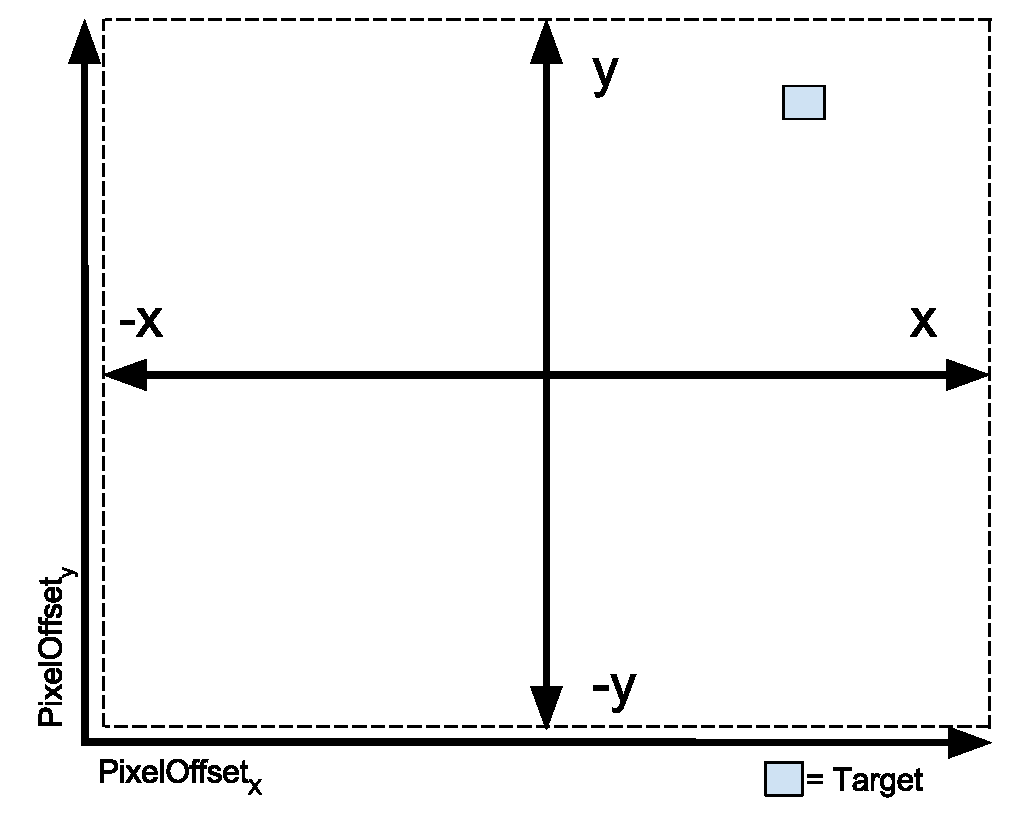
\includegraphics[scale=0.65]{graphics/signed_angles_simple.eps}
    \caption{Example with a marked centre and a target in top right quadrant}
    \label{fig:calculating_angles}
\end{figure}

Using the definition of the x- and y-axis from the image, the z-axis in the 3D room will also have origin in the centre of the lens, but the depth of the image will follow the negative z-axis, resulting in the vector, with tail in the lens, to be defined as
$\left[\!\begin{array}{c}
0\\
0\\
-1
\end{array}\!\right] $
since the vector's direction is away from the lens along the negative z-axis. Before adjusting this vector the deviation along the y- and x-axis must be found. The deviation is found by calculating the fraction of how much the object's pixel is along the two axes. The equations for this are:
\begin{equation}
\frac{Offset_X - 0.5 * Width}{0.5 * Width} \label{eq:offset-x}
\end{equation}
\begin{equation}
\frac{Offset_Y - 0.5 * Height}{0.5 * Height} \label{eq:offset-y}
\end{equation}
\Cref{eq:offset-x} and \cref{eq:offset-y} show the fraction of how far the pixel is along the x- and y-axis, respectively. With the knowledge of these offsets it is possible to calculate the angles for which the vector shall be rotated. A camera has one \acrfull{fov} for each axis. The angles of these \glspl{fov} are used to calculate how many degrees the pixel has moved along the axes. The \gls{fov} is included in \cref{eq:offset-x_fov} and \cref{eq:offset-y_fov}, as $F_x$ for the horizontal \gls{fov} and $F_y$ for the vertical \gls{fov}. Furthermore, the \gls{fov} is halved because the angles are found relative to the centre.

\begin{equation}
\frac{Offset_X - 0.5 * Width}{0.5 * Width}*F_x*0.5 \label{eq:offset-x_fov}
\end{equation}
\begin{align}
\frac{Offset_Y - 0.5 * Height}{0.5 * Height}*F_y*0.5 \label{eq:offset-y_fov}
\end{align}

\Cref{eq:offset-x_fov} and \cref{eq:offset-y_fov} are the final equations that are used for the calculations of the angles. The following section will focus on the rotation of matrices around the x- and y-axes. Lastly an example is given to illustrate the use of the techniques.
\section{Calculating Rotations}
\Cref{ssc:xy_angles} defined how a 2D image is analysed to find the difference, in degrees, between a centred vector and the location of an object. The following section explains how this centred vector is rotated to intersect the targeted object in 3D space.

The angles are found on the x- and y-axis meaning the rotations will be performed on these axes. The rotation matrices needed are shown in \cref{eq:rotation_x} and \cref{eq:rotation_y} respectively.


\begin{equation}\label{eq:rotation_x}
\begin{bmatrix}
1 & 0 & 0 \\
0 & cos\theta & -sin\theta \\
0 & sin\theta & cos\theta \\
\end{bmatrix}
\end{equation}

\begin{equation}\label{eq:rotation_y}
\begin{bmatrix}
cos\theta  & 0 & sin\theta \\
0 & 1 & 0 \\
-sin\theta & 0 & cos\theta \\
\end{bmatrix}
\end{equation}

The rotation matrices rotate vectors counter clockwise from their original direction. \Cref{fig:signed_angles} shows how these rotations are represented in the images.
\begin{figure}[H]
    \centering
    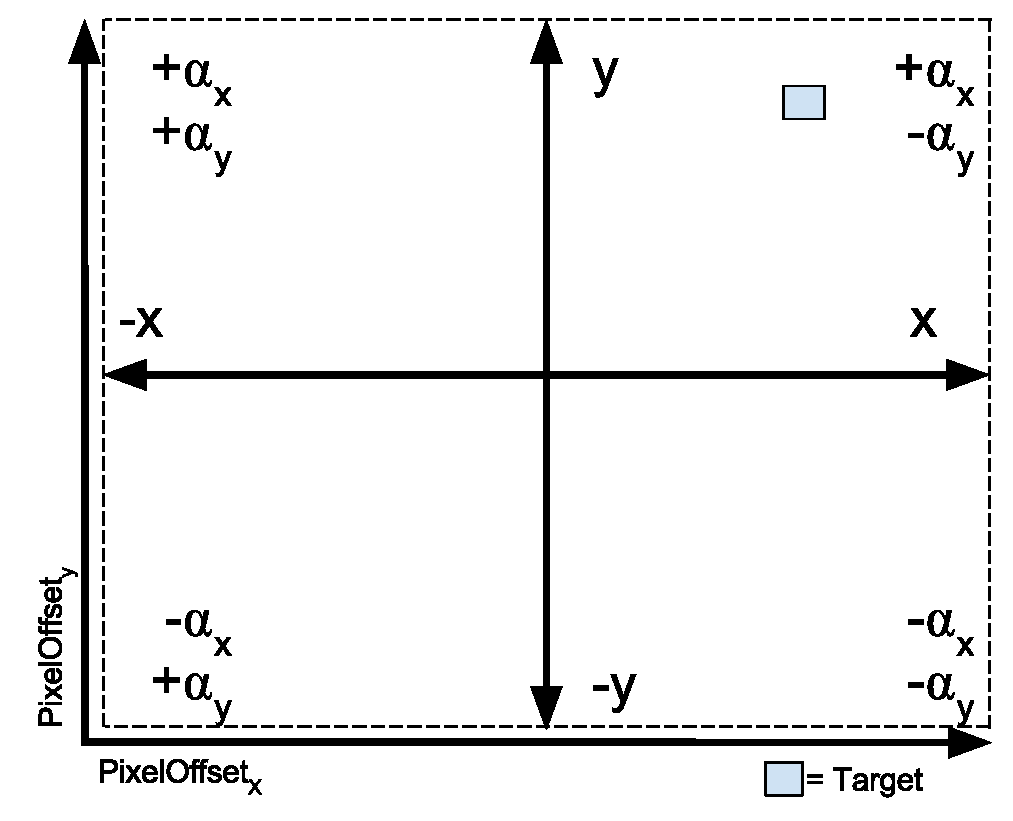
\includegraphics[scale=.65]{graphics/signed_angles.eps}
    \caption{Example showing angle values, depending on graph quadrants}
    \label{fig:signed_angles}
\end{figure}

Looking at the first quadrant containing the target, the rotation around the x-axis must be a counter clockwise rotation from center origin, which is why the degrees must be positive. \Cref{eq:offset-y_fov} returns positive values when target is greater than half the height of the image, therefore, this equation returns the wanted result. \Cref{eq:offset-x_fov} however, returns negative values when target is on the left side of the image and positive values when the target is on the right side of the image, which is opposite from the wanted behaviour. This behaviour is easily achieved however, by negating the result of \cref{eq:offset-x_fov}, resulting in \cref{eq:offset-x_opt}
\begin{align}
-\left(\frac{Offset_X - 0.5 * Width}{0.5 * Width}\right)*F_x*0.5
\label{eq:offset-x_opt}
\end{align}
The following section gives an example of finding the angle derivations and then rotating the lens' centre vector to cut the target's position.

\section{Example of Calculations}
A picture is taken with a camera and an object is defined to be located at the first quadrant of the image, with a pixel offset of $(x,y)=(500,400)$, the size of the image is $640x480$ $pixels$ and the \gls{fov} of the camera is $62\degree$. This information is inserted into \cref{eq:offset-y_fov} and \cref{eq:offset-x_opt}, giving:
\begin{align}
-\left(\frac{500 - 0.5 * 640}{0.5 * 640}*F_x*0.5\right) = -17.44\degree
\label{eq:ex_offset-x_opt}
\end{align}
\begin{align}
\frac{400 - 0.5 * 480}{0.5 * 480}*F_y*0.5 = 20.67\degree
\label{eq:ex_offset-y}
\end{align}

Next is to rotate the wanted vector which is the camera lens' vector previously defined as
$\left[\!\begin{array}{c}
0\\
0\\
-1
\end{array}\!\right] $
 it has to be rotated $20.67\degree$ around the x-axis and $-17.44\degree$ around the y-axis. which is shown in \cref{eq:rotation_on_x_and_y_part1} and \cref{eq:rotation_on_x_and_y_part2}.
\begin{equation}\label{eq:rotation_on_x_and_y_part1}
\begin{bmatrix}
1 & 0 & 0 \\
0 & cos(20.67) & -sin(20.67) \\
0 & sin(20.67) & cos(20.67)
\end{bmatrix}
\begin{bmatrix}
0 \\
0 \\
-1
\end{bmatrix}
=
 \begin{bmatrix}
0 \\
0.353\\
-0.936
\end{bmatrix}
\end{equation}
\begin{equation}\label{eq:rotation_on_x_and_y_part2}
\begin{bmatrix}
cos(-17.44)  & 0 & sin(-17.44) \\
0 & 1 & 0 \\
-sin(-17.44) & 0 & cos(-17.44)
\end{bmatrix}
\begin{bmatrix}
0 \\
0.353\\
-0.936
\end{bmatrix}
=
 \begin{bmatrix}
0.280 \\
0.353 \\
-0.893
\end{bmatrix}
\end{equation}
$\left[\!\begin{array}{c}
0.280 \\
0.353 \\
-0.893
\end{array}\!\right] $
is the vector in the local coordinate system of the camera, which cuts the object. This vector has to be transmuted into the global coordinate, so the actual position of the object can be calculated for the 3D space.

\section{\acrlong{pid} Controller}
\label{ss:pid}
The motors used with the \gls{nxt} are assumed to be cheap in the sense there is no guarantee that an instruction is carried out as precisely as specified. For example, it cannot be assumed that two of the same motors will yield an identical result when instructed to run for a given time frame. The motors are \glspl{dcm}, so it is not possible to instruct them to turn a certain amount of degrees.
To regulate and make sure the motors controlling the targeting device are responsive, as well as carry out the instructions given as precise as possible, it has been chosen to use a \gls{pid} controller. This controller is essentially an algorithm which takes feedback into consideration and compensates for it. It regulates the power at which the motor is working, increasing the power when the motor is far away from its target, and decreasing the power as it approaches the desired angle.  
The mathematical formula for this controller is as follows \citep{pid_controller}:

\begin{equation} \label{pid_formula}
[PID-controller] \
u(t) = K_p *e(t) + K_i \int_0^t e(\tau)d\tau + K_d*
\frac{de}
     {dt}
\end{equation}
There are several adjustable constants denoted by $K$. The algorithm consists of three terms. The first term, $K_p*e(t)$ is a constant multiplied by a tracking error, which is the running difference between the desired input value and the current actual value. The second term, $K_i \int_0^t e(\tau)d\tau$, is a constant multiplied by the running summation of errors. The third term, $K_d* \frac{de}{dt}$, is the last constant multiplied by the difference between the current error and the previous error from last iteration. $dt$ is the interval at which the function is executed in milliseconds, and can be integrated into the three adjustable constants when the controller has a well-defined, confined purpose.

The adjustable parameters all have a specific influence on the controller, as can be seen in table \ref{pid_char}. There are four factors that to some extent are influenced by each of the parameters. Rise time is the time it takes to reach the desired value. Overshoot encodes the degrees of overshoot on the first rise. Settling time is the time it takes to settle itself within a certain range of the desired value. S-S error is short for steady-state error, and is responsible for the difference between the actual final value and the desired value.
These factors are illustrated on the graph shown on \ref{fig:pid_graph} with example values for the parameters.
\begin{table}[H]
\begin{tabular}{|l|l|l|l|l|}
\hline
RESPONSE & RISE TIME    & OVERSHOOT & SETTLING TIME & S-S ERROR \\ \hline
Kp          & Decrease     & Increase  & Small Decrease  & Decrease  \\ \hline
Ki          & Decrease     & Increase  & Increase      & Eliminate \\ \hline
Kd          & Small Increase & Decrease  & Decrease      & No Change \\ \hline
\end{tabular}
\caption{Table showing parameter influence based on \citep[University of Michigan]{pid_controller}}
\label{pid_char}
\end{table}

\begin{figure}[H]
\includegraphics[scale=1]{graphics/pid_graph.png}
\caption{Example graph of a \gls{pid} controllers effect over time with example constant values\cite{pid_controlle_picr}}
\label{fig:pid_graph}
\end{figure}
Using the graph seen on \ref{fig:pid_graph} as an example, the rise time is approximately 0.1 sec, overshoot is 0.3 amplitude, settling time is around 1 second with very little error, and the steady-state error is approximately 0 amplitude. The constants can be fine-tuned to reduce and eliminate these factors.

To be able to adapt the \gls{pid} controller to the \gls{nxt} motors it will be necessary to customize different values for the two motors, as they operate under different loads. The three parameter values are easily found from similar projects, however the different weights on the motors cause this to be a unique case, which incites an alteration. The minimum power for the two motors to operate is different because of the load differences, as explained in \cref{sc:rig}. If this is not taken into account, the controller will never be able to reach its desired value, as it will get close enough for the power value to be beneath the threshold of what the motor needs to operate. Because of this it will be necessary to analyse the output and correct for this case.

\subsection{Termination}
To use a \gls{pid} in a system with real-time requirements it is necessary to impose restrictions on the run-time of the controller. Furthermore, it has to be constructed in such a way that it is possible to determine when the controller has succeeded, meaning the motors are at the desired angles, and the controller is ready for new input. This check can be done by monitoring certain values of the controller; specifically the derivative, which is calculated by finding the difference between the current error and the previous error. It can be assumed that the \gls{pid} has succeeded once the derivative has been equal to zero over a predefined period of time. To strengthen this assumption there can also be checks on the current position of the motors and on the speed of the motor.

A challenge the controller faces is being in charge of two motors instead of one. It is desired that both motors are moving at the same time, as running them in sequence significantly increases the time spent by the controller. Early in the process it became clear that problems arose from two motors running simultaneously. When one motor has finished before the other, the second motor's movement can cause vibrations resulting in the first motor moving a degree away from target. To fix this, a check is added once both motors have finished their movement, confirming the final position is on target. If this is not correct, the controller will iterate over itself once again to fix this error.

The run-time restrictions imposed on the \gls{pid} manifest themselves by a limit on the iterations of the function. After a constant amount of iterations, the controller will be forced to finish even if the target has not been reached. When calculating this amount, the speed of the processor has to be taken into consideration, as a fast processor might be capable of going through all iterations faster than the time it takes for the physical movement. This opens up for the possibility of making worst-case complexity analysis of the controller and schedule it.

\chapter{Motor Test} \label{chpt:motor_test}
As presented in \cref{sec:laser} the laser unit is composed of an \gls{nxt} and accompanying motors which are part of the Lego Mindstorms series. Two of these motors are needed by the laser unit in order to control the laser both horizontally and vertically. It is assumed that the motors are very imprecise and it is therefore necessary to test and analyse the consistency of the motors. The results of the tests can be used to determine which motors are optimal to use and how to handle or even remove uncertainties.

This chapter presents the attributes that the motors are tested for and how the tests are structured. Error sources that could possibly influence the data are presented, and ways of minimising or removing these error sources is described in the structure of the tests. The data from the tests is also presented and analysed in the chapter.

\section{Goals of Testing}\label{sec:test_goals}
The tests are conducted in order to measure three properties; maximum speed, acceleration and brake speed. Besides testing these three aspects the consistency of them all is also tested. The data acquired from the tests is used to determine which motors that exercise the most consistency. There are four motors to be tested, indexed one to four. The number of the motors stays the same throughout the tests, meaning motor 1 is the same motor for all tests.

As explained in \cref{sc:rig}, a total of two motors are needed in the construction of the rig, where these motors are used for the horizontal and vertical axis'. The motors need to turn a pointer in collaboration, to target an object in a 3D room, which affords the need for moving the motors precisely. If a motor has an imprecision of a few degrees, the effect of this imprecision becomes greater as the distance to the target increases. The existence and size of such imprecision and the consequences hereof must be identified when analysing the data.

In order to fulfil the test goals, a single test is conducted which is a speed-timing test. The speed-timing test measures how long it takes to reach maximum speed and how long it takes to get to a full stop from maximum speed. These measurements can be used to obtain the acceleration, maximum speed and negative acceleration. A last aspect is to analyse the consistency of the runs to get an indication of which motors might be the best to use.

\section{Error Sources}\label{sec:error_sources}
A number of error sources are considered while designing and performing the tests, since there is a risk they can have an effect on the results. Some of these error sources occur as a result of using the selected hardware components, as an example there is a significant backlash in the motors. Another source is the test conductor while a third source is the software used to run the test. The sources are put into three categories; human based, hardware based and test structure based sources. These sources can affect the conclusions of the conducted tests and therefore the associated challenges must be identified.

\subsection{Human Based Sources}
A human based error source is the test conductor. Involving a person in a test may result in human mistakes being made, for example wrongly recording test data or not strictly following the test procedure. By automating tasks, and creating precise descriptions of the test procedures, this uncertainty can be eliminated. But as soon as a person is involved, the uncertainty cannot be entirely eliminated.

\subsection{Hardware Based Sources}
Two hardware based error sources manifest themselves in motor backlash and the internal counter. Because of the quality of the used motors, the precision of their internal components or the size of the backlash cannot be guaranteed.

The first source is the backlash in the motors. It is important that there is a test procedure that either minimises this backlash or makes it a constant value. If this source can be minimized it is more preferred than having a constant factor of backlash in the measurements. Having a constant value for backlash makes it possible to adjust the data if this is known. A problem is that the size of a constant factor can be hard to determine if other error sources are present and therefore the data will be harder to be proper analysed. Therefore it is preferred that the backlash is minimised since the size of the backlash must be obtained.

The second source is internal counter of the motors that counts the number of ticks the motor has moved in a given direction and there might be uncertainties when it reads the tick value. This source is hard to eliminate since it is the equipment used for measuring how much the motor has moved. The size of this reading uncertainty can be estimated if the backlash is eliminated. If backlash is not eliminated the combined effect of the internal counter of the backlash can be measured.

\subsection{Test Structure Based Sources}
There are three error sources that are based on the test structure and test setup. The first is rig structure, which is described in \cref{sc:rig}. The motors are tested while being integrated in this construction.

By including the motors the conditions for the test is the same as when the motor is implemented in a solution. The motors will pull the same weight as if they were included in the final version. This results in data that gives a better foundation for determine which motors are best. A problem is that the construction of the rig can differ between tests of motors. If it does the motors might pull different weights which might affect the data. Two things can be done to minimise this source's impact; having a clear definition of the rigs structure and to have a single test conductor. The last might result in the same structure in all tests but might not be enough to eliminate this source.

A second source is errors in test software. The used software can contain errors resulting in unexpected behaviour. These errors might not be observable while running the test. Therefore the test software should be validated and its behaviour should be tested so it pays respect to its specification, and thereby securing its correctness.

\subsection{Handling Error Sources}
Most of the error sources can either be minimised or eliminated if the test procedure is properly structured, defined and executed. The impact of the sources can be analysed when the results of the tests is obtained. By having identified these error sources it must be part of the data analysis to determine whether or not they had an influence on the data and if so to what extend.

\section{Speed-Timing Test}
In \cref{sec:test_goals} one test was defined as a speed-timing test. This test's purposes are to measure the time used to meet maximum speed, what the maximum speed is and how long time it takes to reach a full stop. This section then presents the test's hypothesis, test structure, data analysis and conclusion.

\subsection{Hypothesis and Test Structure}\label{subsec:acc_test_hyp}
Before presenting the structure of the test structure a hypothesis must be defined. The structure is based in the hypothesis since the data must prove or disprove the hypothesis where the hypothesis is based on the purpose of the test. The hypothesis for this test contains three parts:
\begin{enumerate}[label=\alph*)]
    \item The speed before the motor reached its maximum speed is linear in growth.
    \item When maximum speed is reached the speed will be constant, and not oscillating, until the motor is instructed to brake.
    \item The negative acceleration when braking is linear.
    \item The motor's positive and negative accelerations are the same size.
\end{enumerate}

The three parts are based on assumptions of how the data is formed. In order to prove of disprove the claims the test structure is designed to measure the distance covered at any point in time. From this data the speed can be obtained and from speed the acceleration can be obtained. Having this information the four parts of the hypothesis can be proved or disproved depending on the results.

The hardware used for this test are the \gls{nxt} from the \acrlong{nxt} series, motors from the same series and the rig constructed in \cref{sc:rig}. The \gls{nxt} used the battery pack from the series which delivers 7.4V. The battery pack is connected to charger. The motor to be tested was included in the setup as the motor responsible for the vertical rotation. Doing so the motor have the weight of the other motor. The alternative was that the motor would not have any weight but this might give other results than having the weight on since less momentum is needed.

The software written for this test had the following structure:
\begin{enumerate}
	\item The tick counter is set to zero.
    \item The motor is instructed to run at full speed.
    \item At every millisecond the tick counter is read and the value stored.
    \item At 250 milliseconds the speed is set to zero and the brake is activated.
    \item At every millisecond the tick counter is read and the value stored.
    \item The test stops at 500 milliseconds.
\end{enumerate}
The test software can be seen in \cref{lst_speed_timing} in the appendix.

This procedure was repeated 250 times for each of the four motors that are available. In order to save the data every test was saved in memory on the \gls{nxt}. When the test was finished the data was send to a secondary device for storage. By doing so there was not writing to secondary memory during the tests but in between the tests. Also it reduces the risk that the test conductor makes errors since he only set the tests up and the rest is automated.

The motors are instructed to turn the same way in every test which reduces the influence of backlash. The first test's data might be altered  but the later tests will start from a position where the backlash is minimised. The source that might have the largest impact is the rig construction. If the rig is not properly put together when the motor is changed the data from the different motors might give very different results. This could remove the possibility of getting trustworthy data.

The presented test structure of the speed-timing test is based on four parts of the hypothesis. Error sources are reduced and the data analysis in the section below must determine whether or not the reduction is a success.

\subsection{Data Analysis}\label{ss:data_anal}
The test structure for the speed-timing test gave 250 data sets. This gives 250 data points for each millisecond. In order to work with this the median value for each data point was selected so there instead was one data point for each millisecond. This data set can easily be plotted and a fit can be made.  Then it can be determined if the accelerations is linear in growth. The test software used to record these data points have been reviewed multiple times and been deemed sufficiently correct to guarantee the data to be acceptable for analysing the motors. All figures shown are for motor 1 but all figure for all motors can be seen in \cref{app:res}.

In \cref{fig:data_fit_1} the data for motor 1 is plotted together with a piece wise plot fit. The figure shows the number of degrees the motor has moved at each millisecond, which gives the distance covered at any given time. The data points until maximum speed have a polynomial fit of second order and the same is the data points at negative acceleration. When maximum speed was reached it is linear fit and the same when the brake is finished.

\begin{figure}[!htb]
    \centering
	\includegraphics[width=1\textwidth]{test_res/speed_tests/Data_and_fit_motor1.pdf}
     \caption{Test data for motor 1 for the speed-timing test}
	\label{fig:data_fit_1}
\end{figure}

It is no surprise that it is a linear fit when the brake is completed since no more distance is covered. This function for this fit for all for motors is just a constant where the constant is the mean value of the data within the fit's data range. The first increase in instance and when braking are both fitted with a polynomial fit of second order which is consistent with constant acceleration. The distance covered after maximum speed was reached until the brake is introduced the fit is also linear. All of fits made for all the four motors have an R\textsuperscript{2}-value that is above 0.99. Having such a high value means that a fit of higher order is not needed. Now having these piece wise plot fit consisting of four parts it is possible to analyse the speed speed at any given moment. The plot fit was differentiated and is shown in \cref{fig:speed_1}.

\begin{figure}[!htb]
    \centering
	\includegraphics[width=1\textwidth]{test_res/speed_tests/Speed_motor1.pdf}
     \caption{Speed at any given time for motor 1 for the speed-timing test}
	\label{fig:speed_1}
\end{figure}

One thing to notice is how the first plot fit crosses the y-axis and does not cross point $(0,0)$. This is due to fit not being a perfect fit but since the R\textsuperscript{2}-value is above 0.99 this is accepted. The plot might have a better fit if the order was higher and therefore start in point $(0,0)$. A problem that could arise by having a higher order is when the fit is differentiated to get the speed and the acceleration. By having a higher order the speed and acceleration could appear to oscillate in the tests. This fluctuation might be unobservable if a very high order is used and it would give a more smooth transition between the four functions used to fit the data in \cref{fig:speed_1}. Otherwise the second order fits have a good fit on the data so it is determined that a second order fit is sufficient for analysing the data.

\begin{table}
  \centering
  \begin{tabular}{| c | c | c |}
    \hline
    Motor Id & Max speed reached at & Max speed in Degrees/ms   \\ \hline
    1 & 95 ms & 0.723 \\ \hline
    2 & 95 ms & 0.723  \\ \hline
    3 & 100 ms & 0.730 \\ \hline
    4 & 94 ms & 0.716   \\ \hline
  \end{tabular}
  \caption{The maximum speed for the speed timing test}
  \label{tbl:max-speed}
\end{table}

From \cref{fig:speed_1} and the plot fits for the three other motors the maximum speed is obtained. In \cref{tbl:max-speed} the time taken to reach maximum speed is listed including the speed itself. Motor 3 is the only motor that notably differs from the other motors in the time it takes to reach maximum speed. Otherwise it is noted that the might be a relation between the size of the speed and the time it takes to reach it. The less time used to reach the speed the less the speed is. This speed does not make it clear which motors to use. The distance the motors cover in 10ms at maximum speed is 7.x degrees. The resolution for internal counter is 1 degree so the difference would be unobservable. If the motor are on for a longer time the difference would be observable but acceleration and consistency of the motors must be determined before the maximum speed can be used.

\begin{figure}[!htb]
    \centering
	\includegraphics[width=1\textwidth]{test_res/speed_tests/Acc_motor1.pdf}
     \caption{Acceleration at any given time for motor 1 for the speed-timing test.}
	\label{fig:acc_1}
\end{figure}

The acceleration for motor 1 is shown in \cref{fig:acc_1}. The acceleration is constant for all four piecewise plots. The acceleration when maximum speed and full stop is reached is 0 since the speed in constant. In \cref{tbl:acc} all the positive and negative accelerations are presented. Every motor's positive acceleration is greater than its negative acceleration. The ration between the motors' two accelerations are between 0.90 to 0.94. Therefore it can not be said that in the general case that the accelerations are of the same size.

\begin{table}
  \centering
  \begin{tabular}{| c | c | c |}
    \hline
    Motor Id & Positive acceleration in degrees/ms\textsuperscript{2}& Negative acceleration in degrees/ms\textsuperscript{2}  \\ \hline
    1 & 0.00712 & -0.00637 \\ \hline
    2 & 0.00701 & -0.00662  \\ \hline
    3 & 0.00677 & -0.00630 \\ \hline
    4 & 0.00703 & -0.00636   \\ \hline
  \end{tabular}
  \caption{The positive and negative accelerations for the speed timing test}
  \label{tbl:acc}
\end{table}

Before concluding on any of the data the standard deviation is considered. In \cref{fig:standard_1} the standard deviation for motor 1 is shown. For the most part the deviation follows a linear growth up until the 300 milliseconds mark which suggest a constant value being applied every millisecond. For all four motors there is a high increase in deviation for the first 10 milliseconds where there rise becomes linear. When the motors is instructed to brake the size of the increase falls and there is no longer any increase when the motors has reached full stop. This means that increase in deviation is linear in time at maximum speed and while the motors has a positive acceleration.

Backlash does not explain why the deviation increases over time. It would explain a deviation the first data point was read but after that the motor would have moved past the backlash. An increasing in deviation could indicate that the constant values for speed and acceleration changes throughout the test runs. If two tests have different values the difference in distance covered would increase as more time parses. As the difference increases over time the standard deviation would do the same. If the values are different between test runs the voltage delivered to the motor has changed between tests. The tests was done with a battery pack connected to the charger. Since the battery pack is a lithium battery the voltage decreases over time. Running tests lower the battery charge but the battery would when be charged, which could result in an oscillating size of voltage. A change in 0.005 degrees/ms\textsuperscript{2} gives a difference of 1 degree after 200 milliseconds which would require an increase of 5-6\textperthousand\ is needed. Since only a small change in voltage is needed to create the observed deviation an oscillating voltage could be the error source.

Another source explaining the increases of standard deviation over time could be the internal tick counter in the motors. If the counter has a constant risk of missing a tick it would result in a linear growing standard deviation. This error source is far less preferable than having a battery pack that changes it voltages. If ticks are missed by the counter it is not possible for the counter to observe the miss and thereby recover from it and the motors might be calibrated more often. If the source for changes in deviation is the battery pack the power source can be changed to a constant voltage which would remove the linear growth in deviation.

\begin{figure}[!htb]
    \centering
	\includegraphics[width=1\textwidth]{test_res/speed_tests/StandardDeviation_motor_1.pdf}
     \caption{Standard deviation at any given time for motor 1 for the speed-timing test}
	\label{fig:standard_1}
\end{figure}

\subsection{Conclusion of Speed-Timing Test}\label{subsec:con_speed}
After reviewing the data, it can be seen that all but one of the presented hypothesis holds. The speed before the motor reached its maximum speed was measured to be of linear growth. When maximum speed is reached the speed is constant until the motor is instructed to brake and since the plot fit had a R\textsuperscript{2} of 0.99 the speed is considered to not oscillate. The negative acceleration when braking was measured to be of linear decline. The motors' positive and negative accelerations ratio is too different as the ratio between the accelerations are 0.90 to 0.94.

There is no clear indication of which motors are better than the others from this test. Their values for acceleration and top speed are close to each other. One aspect to where their differ is in standard deviation. If the increase in standard deviation is caused by skipping ticks no amount of calibrating will be successful as the model rapidly deviates from reality. This deviation results in frequent need of calibration if the internal tick counter is used. Rather using the tick counter external means could be used to measure the distance the motor covered.

If the error source is not the tick counter but rather changes in voltage a \gls{pid} as presented in \cref{ss:pid} would compensates for the deviation. This compensation occurs since the \gls{pid} continually approaches a target value. It is estimated that changes in voltage has a higher probability to be the source of errors than the tick counter. If this assumptions holds there is no need to conduct more tests as the \gls{pid} compensates for the motors' standard deviation. If the standard deviation is removed no motor can be said to be better then the others. But considering the deviation motor 3 has a standard deviation of 2.5 where the others deviation is about 1.7. Therefore motor 3 would be the least preferable to use.
\chapter{Implementation of \gls{pid}}
\label{ss:pid_imp}
The \gls{pid} controller has been challenging to implement because of several aspects. First of all, there is no predefined way of ensuring termination. Several different methods have been attempted, including having a simple integer value counter and testing whether the motor has been at the same position several iterations in sequence. As mentioned in \cref{ss:pid}, it is also desired to have both motors running simultaneously, which incites a check at the end, to ensure both motors are static at the correct position.

The algorithm for the controller is very simple and it is easy to find examples on how to implement it. However, a layer of program logic has been added to ensure controlled usage of the algorithm. This section will show parts of this layer, and how termination has been ensured for use in a system with real-time requirements.

The \gls{pid} controller uses four functions. The prototypes can be seen in \cref{lst_pid_functions}. The first function, $move\_motors$, is the function that is initially called and simply takes two angles as formal parameters. This function calls $motor\_pid$ a number of times for each motor, which calculates a new speed using $pid$ and sets the motor to this speed. The final function, $min\_speed$, is an auxiliary function which simply looks up a motor id and returns a value for the minimum speed of that motor.
\begin{lstlisting}[language=inc_cpp, caption={Prototypes for the \gls{pid} functions}, label=lst_pid_functions]
void move_motors(S32, S32);
S32 motor_pid(S32, U8, S32[], S32[], S32[]);
S32 pid(S32, S32, S32*, S32*, S32*, U8);
U8 min_speed(U8);
\end{lstlisting}

The $pid$ function is shown in \cref{lst_pid}. It calculates a value using the algorithm presented in \cref{ss:pid}. An alteration has been added, such that the return value of this function considers the algorithm output against two thresholds.  These thresholds are illustrated on \cref{fig:pid_threshold}. The first threshold, $PID\_SPEED\_MIN\_VALUE$, is used to check that the function returns zero when there is a strong indication that the motor is on target. The second threshold, $minspeed$, is the minimum power for the motor to run. If the algorithm outputs a value higher than the first threshold and lower than the minimum power threshold, the return value of the function will be the minimum power threshold.
\begin{lstlisting}[language=inc_cpp, caption={The pid function}, label=lst_pid]
S32 pid(S32 target, S32 current, S32 *integrale ...) {
    ...
    float speed = (error*KP + KI*(*integrale) + KD*(*derivative));
    U8 minspeed = min_speed(motor);
    ...
    return (speed > 0 && speed < PID_SPEED_MIN_VALUE) ? 0 :
           (speed < 0 && speed > -PID_SPEED_MIN_VALUE) ? 0 :
           (speed > 0 && speed < minspeed) ? minspeed :
           (speed > -minspeed && speed < 0) ? -minspeed :
           (S32)speed;
}
\end{lstlisting}

\begin{figure}[H]
\includegraphics[scale=1]{graphics/speed_diagram.eps}
\caption{Illustration of the return statement for the function $pid$ as seen in \cref{lst_pid}}
\label{fig:pid_threshold}
\end{figure}

The function called $move\_motors$ has the responsibility of performing the iterations while also ensuring termination. This is done by using two nested loops. In the inner loop, two separate if-statements are repeatedly evaluated. The if-statement responsible for the horizontal motor can be seen on \cref{lst_move_motors1}. First, a new speed is calculated and set for the horizontal motor. There are three cases in which it is desired to use the brake on the motor and mark the \gls{pid} as finished with this motor. The first and most important case is if too many iterations have been used. The second case is the conjunction of the motor being at the right tick, the speed being zero and the previous speed being zero. A special case was added to eliminate settling time when the laser has to be moved very little. This last case comes into play when the function is called with arguments stating the motor has to rotate very little, because it is close to its target. This is assumed to happen a lot when tracking moving objects, and the case eliminates unnecessary time spent settling.
\begin{lstlisting}[language=inc_cpp, caption={The \textit{move\_motors} function}, label=lst_move_motors1]
if(horisontal_fin == FALSE) {
    speed_horisontal = motor_pid(horisontal, HORISONTAL_MOTOR, 
                                 integrale, lastError, derivative);
    if(counter_horisontal++ >= limit_horisontal || 
      (nxt_motor_get_count(HORISONTAL_MOTOR) == horisontal && 
       speed_horisontal == 0 && derivative[HORISONTAL_MOTOR] == 0)|| 
      (diff_horisontal <=3 && 
       nxt_motor_get_count(HORISONTAL_MOTOR) <=horisontal+1 && 
       nxt_motor_get_count(HORISONTAL_MOTOR) >=horisontal-1)){
        motorA.setBrake(1);
        horisontal_fin = TRUE;
    }
}
// Similar if-statement for the vertical motor.
\end{lstlisting}
These two if-statements are executed in sequence for as long as the motors have not been marked as finished. Once both motors are marked as finished, the outer loop will reset certain auxiliary variables and another iteration of the inner loop will be performed to ensure that the laser is correctly angled. 

It is important to note that the time spent in the inner loop is reduced significantly when the motors are near the desired target. This means that the overhead of running the inner loop one or two times too many, is insignificant. Because of this it has been chosen to run the outer loop a constant amount of times, which allows for the possibility of calculating the complexity. The worst-case complexity for the nested loop is then calculated by simply multiplying the limit from the first case in the if-statements by the amount of times the outer loop is iterated over. This worst-case is an overestimate, as it is unlikely that both loops uses the highest possible iterations.

\chapter{Discussion}
\label{chpt:discussion}
This chapter will review the choices that have been made throughout the project, while reflecting on other possible choices and what consequences they would have on the product.

\section{Requirements}\label{sec_disc_requirements}
A set of requirements was specified and categorised as either must have, good to have or stretch goals. Two requirements were categorised as must have: \textit{Object Recognition} and \textit{Target Tracking}.

The requirement of \textit{Object Recognition} is fulfilled trough \gls{opencv} which makes it possible to recognise a predefined object, by the use of template matching. 

The rig was built in order to provide the Lego Mindstorms motors with a base of which they can perform horizontal and vertical rotations, to move a laser around to point in specified directions in the room, in which it is located.
The \gls{nxt} controls these motors and can thereby adjust the direction of the laser, and therefore track the recognised object by aiming the laser at the object.
By doing combining these elements the second requirement, \textit{Target Tracking}, has likewise been fulfilled.

Advanced Target Acquisition have not been implemented in the system. However, the system accepts position information in a general form, meaning the changes that are to be done for the system to accept positions from more than two cameras is minimal. By including this option new obstacles are introduced, as the system would have to discard redundant information, as there are more candidates to specify the object's position. Information can be deemed redundant if the position it specifies is too distant from the set of collected positions. This situation can occur if a camera recognises a wrong object or somehow corrupt the data it sends. Furthermore, by having more candidates, the information can be evaluated, to find possible errors.

\section{Hardware}\label{sec:disc_hardware}
The choice of hardware have brought different implications and restrictions on what is possible when designing the system. Some of these implications could have been avoided by using different pieces of hardware, but these devices would have their own restrictions as well. This section will discuss the possibilities and restrictions of altering the hardware choices and setup.

\subsection{Mindstorms Devices}\label{subsec:disc_minds}
The \gls{nxt} is used to calculate the angles that the rig adjust itself to when instructed to point at a target, and the \gls{rsp} is responsible for the analysis of images from the camera video streams. There is a newer version of the nxt called \gls{ev3}. If the newer Mindstorms brick was used, it would be possible to offload the calculations from the \gls{rsp} to the brick as it has more computational power. As seen in \cref{tbl:ev3_spec} the \gls{ev3} has a faster processor along with a large increase in the amount of memory it has access to. It should be noted that the power consumption is increased as well.

\begin{table}[ht]
  \centering
  \begin{tabular}{|l|r|}
  \hline
    Main processor & 32-bit ARM9 processor, Texas Instrument AM1808\\ \hline
    Memory & 64 MB DDR RAM, 16 MB FLASH, 256 KB EEPROM\\
  \hline
  \end{tabular}
  \caption{Summarised \gls{ev3} intelligent brick specification\cite{ev3_specs}}
  \label{tbl:ev3_spec}
\end{table}

By offloading these calculations to the \gls{ev3} it would be possible to replace the \glspl{rsp} with a simpler device, which transfers the video stream directly to the \gls{ev3}. This solution will also allow the system to spare the laptop as it will not be necessary to have an intermediate component to act as modem.

\subsection{No PC and Lego Mindstorms NXT Solution}\label{subsec:disc_no_pc_lego}
In the current system setup, a total of three different devices are used, namely a \gls{nxt}, \gls{rsp} and a laptop, each running a different \gls{os}. If a newer version of the \gls{rsp} was used, such as the \gls{rspz}, it would be possible to create a system of unified devices which would widen the communication possibilities. The \gls{rspz} is a cheap embedded device with normal and mini USB ports and can be modified to connect trough an Ethernet connection as well. The \glspl{rsp} have their own set of motors which is found in a varying price and quality range, which could be used instead of the Lego Mindstorms motors.\cite{rs_pi_zero} \cite{rsp_zero_ethernet}

If the system, besides the sensors and actuators, only consisted of \glspl{rspz}, the communication process would be simplified, since the amount of different \glspl{os} and devices the project group would have to familiarise themselves with would be reduced.

\subsection{Modern Camera Possibilities}\label{subsec:disc_modern_cam}
%Newer cameras will allow better precision and the object reg will be more effective
%	(Bedre template - små objekter - chance for rigtigt - ansigtsgenkendelse)
In \cref{ss:cam_type} two camera options are presented and as stated the \acrfull{cvbw3} is selected. However, since the release of \gls{cvbw3}, the quality of webcams have been enhanced, including the quality of the images. This quality increase manifests itself in higher resolution, a larger point of view and a higher degree of details in images.

These quality enhancements are relevant in relation to object recognition as presented in \cref{ch:obj_rec}. This is due to the higher degree of details in an image as it makes it easier to distinguish elements, resulting in easier object detection and recognition.

\subsection{Multiple Cameras per Raspberry Pi}\label{subsec:disc_mult_pi}
%Why not use two or more cams per PI? (answer: ram)
As the system is designed, each camera unit is constructed using a \gls{cvbw3} and a \gls{rsp}, both presented in \cref{chp:tech}. An alternative setup would be to equip each \gls{rsp} with multiple \glspl{cvbw3}. There are both advantages and disadvantages to such a solution. The advantage is a decrease in the amount of hardware needed in total, as two cameras can be connected to a single \gls{rsp}, such that it is possible to half the amount of \glspl{rsp} needed. However there is a disadvantages to this approach in relation to the range of the cameras units. This is due to the USB specification, which states that a USB cable's length should at maximum be 5 meters, otherwise a decrease in transfer speed may occur \cite{usb_spec}. While a Ethernet cable can be up to 100 meters before a decrease in transfer speed may occur. By using two cameras per \gls{rsp}, the amount of hardware per unit will decrease, but more units are needed to cover the same area.

\subsection{Alternative Motor}\label{subsec:disc_step}
The motors used are \glspl{dcm} which are controlled by regulating the voltage they receive. As a consequence of this method it is not possible, by standard, to instruct the motor to rotate a set amount of degrees. Therefore a \gls{pid} has been implemented in order to rotate the correct amount of degrees. It would be possible to avoid the implementation of a \gls{pid} if a step motor was used, as it can be instructed to rotate a set amount of steps. It would simplify the implementation and make the system react faster as it would not have to call a \gls{pid} function when instructed to rotate. However, step motors are generally very expensive when compared to their \glspl{dcm} counterpart. 

\section{Implementation}\label{sec:disc_implementation}
When implementing the mathematical formulas and getting them to work with a real life environment, different problems arise which have to be handled. One of these comes from how the rig has been designed and what that entails. How the object recognition have been implemented also provides a set of dilemmas when working with multiple cameras.

\subsection{Rig Design}\label{subsec:disc_rig}
When calculating the angles, there is an offset that has to be considered because of how the rig is constructed. There are two axes each represented by a motor which is used to angle the laser in the right direction when an object has been targeted. \Cref{fig:rig_flat} from \cref{sc:rig} shows where the offset is. From the turret base vertical centre line, the centre of the big gear, to the axis that makes the vertical rotation there is a distance of 6,4cm which form the offset.

If the rig was build in such a way such that the two axes had the same rotational point, it would not be necessary to include an offset in the calculations. This can be achieved by using a gimbal setup with the laser in the centre.

\begin{figure}[H]
  \centering
  \includegraphics[width=0.80\textwidth]{graphics/discussion/gimbal.jpg}
  \caption{Gimbal example\cite{gimbal}}
  \label{fig:gimbal}
\end{figure}

If the laser was fastened in centre of the gimbal from \cref{fig:gimbal}, it would be possible to eliminate any offsets if the coordinate system would have its base in the centre as well. This would simplify the angle calculations and make them more precise, as the possible imprecisions made when measuring the offset will be eliminated as well.

\subsection{Multiple Camera Tracking Dilemma}\label{subsec:disc_mult_cam}
In order to find and track an object with the current setup, it is necessary that all connected cameras have targeted the same object. If one or more cameras are unable to target the same objects as the other cameras, the result is undefined. What will probably happen is that the calculated angle on the \gls{nxt} will be inequivalent with the angle of the correct target. If a camera unit is unable to find and target an object, the pixel offset is undefined, which will cascade to the following calculations. When an objects position is calculated on the \gls{nxt}, all the information retrieved from the pc is used, which means if one of them delivers erroneous or otherwise nonsensical data the calculations will be inaccurate.

This could be avoided if the \gls{nxt} was able to discard results that are over a set margin in order to weed out said erroneous data. By discarding wrong data the \gls{pid} will be faster and more precise as it will no longer have to rotate towards a wrong direction, and instead it can use the most recently accepted data packet.

%Simon har læst hertiltiltiltiltiltil. ok siiiimon xD
\section{Test}
\label{sec:disc_test}
\Cref{chpt:motor_test} covers the tests that was conducted with the activators that are used with the rig, but contains no references to the sensors which have been used in the project. The cameras are the choice of sensors when an object has to be recognised and tracked, it would therefore be beneficial for the project to test the quality and limit of these cameras. The produced software have not been tested either, besides small simplistic undocumented test made to ensure that bits and parts gave expected results while they were still being developed. The following sections will describe which additional tests that could have been beneficial for the project.

\subsection{Camera}\label{subsec:disc_camera}
The tests made on the cameras will help to estimate the quality and thereby the chance of the finding the right objects when executing the object recognition software.

Four tests were considered for the cameras where each test would cover different aspects of the devices usability. The four tests were:
\begin{itemize}
\item Verification test of the \gls{fov}
\item Test of the how well cameras fares in different light levels
\item Test of picture noise
\item Test of picture frame rate consistency
\end{itemize}

The Verification test of the \gls{fov} is relevant as the target tracking calculations is dependent on this property. If these calculations returns incorrect angles, it can prove difficult to find where the mistakes were made since no tests have been conducted, and it is therefore not possible to exclude the possibility of having a wrong \gls{fov} constant. The test setup would be to place a camera a set distance, 2-3 meters, away from a blackboard. The camera should point at the centre of the board, and the board should face the camera such that a 90\degree angle from the board would point at the centre of the camera lens. The board will then be chalked up with vertical lines representing where the camera should be able to see within its \gls{fov}. The camera then takes a picture which will be inspected, and if the lines is not in the outskirts of the picture additional lines should be made with a set amount of degrees between them so the actual \gls{fov} can be measured.

The test that inspects how well the cameras fares in different light levels would be helpful as the light level will affect how the colour recognition performs. If it is much darker or lighter than what it is in the template it can be unable to find the target. The template is the reference picture of the object it has to find. It is possible to create many test scenarios that concerns itself with different kind of light setup which test many different aspects of the object recognition. The test that was considered would focus on colour aspect as the light source would be the same, but the light level would be different from what it was at the time the template picture were made. The test setup would be to place the object at the same location that the template picture were taken at, and the keep adjusting the lighting level so keeps getting darker. A camera would point at the object and a device will execute the object recognition software on the video stream. When it no longer is able to consistently find the object, the light level will be noted.

The test of picture noise would be beneficial, as it would provide insight in what techniques that should be used to counter the level of noise present in the pictures. The techniques will complicate the object recognition as more steps are required in order to recognize the correct object. The setup would involve placing the camera in a room where the environment is static in the sense that nothing is moved in between the frames. It is important that the camera is standing still and that the light level stays the same as these factors will affect the result of the comparison made between the frames. The comparison is between two or more frames where each pixel in said frames is compared in order to spot differences. The pixel differences is then counted and compared to the total pixel count in a frame to calculate the \textperthousand difference.

The last test with the cameras would be to test the frame rate consistency. In other words, to check if the time frame between each transfer to the connected device is the same. The consistency is important when calculating a \gls{rta} as any inconsistencies will affect the rate which the devices connected to the cameras can perform their calculations and transfer that data. The test setup would be to connect a camera to a device. The device would then execute a program that timestamps the frames it receives from the video stream. The timestamps would then be compared to find any inconsistencies between the time it takes to receive each picture from the stream.

\subsection{Motor Test}\label{subsec:disc_motor}
in \cref{chpt:motor_test} one test was described and the results was analysed. One problem with this test was that two possible error sources could have affected the standard deviation, as presented in \cref{subsec:con_speed}. Therefore it could be beneficial to conduct two more tests; one for testing the internal tick counter and one for testing the size and speed under constant voltage.

It would be prudent to perform the Speed-Timing Test, where the test setup is connect to a power source where a constant voltage is guaranteed, and not a power source which discharges over time. Such a test could determine the effect a constant power source have on the test results. If it turns out that a constant voltage removes the linear growth in standard deviation, other tests could be a benefit to conduct. The effect of lowering the voltage could systematically be tested so it was known how the motor performs at given voltage.

Another aspect is to test if the battery pack used in the test could oscillate so much it would be observable in the standard deviation. This should be done such that it is understood how the battery pack charges and discharges, and by such the battery based power source influence on the recorded test results. These results should be combined with the results of testing with constant voltage in order to conclude the effect of the standard deviation.

The last test to conduct is to compare the internal tick counter with how far the motors actually turns. The motors have an intern tick counter which counts how many degrees it have turned around its axis. The counter should be that one tick correspondence one degree. The counter is used when turning the laser and will therefore affect how well it will be able to point at a target. The test setup would be to have extra equipment to measure the degrees turned and compare it with the tick counter. If there is a constant risk of skipping it can be observed in the results.


\subsection{Software Test}\label{subsec:disc_software}
During the system development phase, no structured software test were implemented. However it would be an advantage to implement structured test of the source code, as this would make it possible to prove the correctness of the source code. Using test coverage tools developers and testers could get an overview over the parts of the source code which are not yet tested, and which parts of the source code that already are included in the structured tests.

If a structured software test is implemented, it would not only make it possible to prove the correctness and provide test coverage of source code. A structured test would also enable quality control of the source code, thus ensuring the source code lives up to certain quality control attributes. Implementing a comprehensive quality control procedure is an greatly excessive undertaking, but should result in a better product as it would uphold certain criteria and quality control attributes.
\chapter{Conclusion}
% Hvad har vi lavet?
In the course of this project we have build an ILBS which is capable of delivering indoor positioning data in real-time from Wi-Fi devices inside a set perimeter. This is done utilising a RESTFful service to communicate with a Cisco MSE service from which we are able to transfer and process the captured data. After the data is processed it is send to a database of which other aSTEP developers are responsible for. The data can then be requested by the different application and API developing groups.

% Sprint 1
In order to acquire mock data for aSTEP we chose to integrate MSE for the indoor positioning system as it was the most convenient choice. MSE was already installed at campus and the functionality it offers was sufficient to our needs. The data is processed and modified before it reaches the database as we had to obfuscate some of the sensitive personal data. It was decided to do so partly because of a request from the campus MSE administrator and due to the Danish law of \textit{Directive on privacy and electronic communications}. As of such it was decided to obfuscate the person sensitive data of those users that did not consent.

% Sprint 2
The client that was build is intended for acquiring data from multiple MSE services, as well our intimidate server, and for sending data to the database. The client was designed to be robust and flexible, which was achieved by providing it with mechanisms for handling errors and by implementing a RESTful service for user inputs. 

% Sprint 3
The foundation for a small tracking system was laid, with the future goal of being comparable with MSE in terms of the precision of the geographical coordinates. % Hvad er der mere at sige?

% Sprint 4 + resten
In order to give future students an easier start, when they take ownership of the project, a set of precautions have been made. This involves code documentation, code tests, the section \nameref{sec:catchup} and the various "How-to"s that have been made for this project's wiki at GitLab. 

% Konklussion 













































































%%%% Appendiks %%%%
\appendix														% Appendiks/bilag start - giver chapter bogstaver i stedet for tal
\clearforchapter												% Sikrer at pagestylen aktiveres paa den rigtige side
\phantomsection													% Kunstigt afsnit, som hyperlinks kan 'holde fast i'
\pdfbookmark[0]{Appendiks}{appendiks}							% Tildeler en klikbar bookmark til den endelige PDF
\chapter{Speed-timing test software}
\begin{lstlisting}[language=inc_cpp, caption={Speed-Timing Test software}, label=lst_speed_timing][H]
#include "Lcd.h"
#include <Nxt.h>
#include <Clock.h>
#include <Usb.h>
#include <math.h>
#include <Motor.h>
#include <vector>
#include "kernel.h"
#include "kernel_id.h"
#include "ecrobot_interface.h"
#include "my_constants.h"

#define TIME_INTERVAL 1
#define TEST_COUNT 250
#define DATA_POINTS 750

using namespace ecrobot;

extern "C" {
    // nxtOSEK hook to be invoked from an ISR in category 2
    void user_1ms_isr_type2(void) { }
    
    void prepare_packet(char packet_type, char *data, U8 *out, int count) {
        out[0] = packet_type;
        for (int i = 0; i < count; ++i) {
            out[i+1] = data[i];
        }
    }
    Clock clck;
    Lcd lcd;
    Nxt nxt;
    Usb usb;
    Motor mtr(PORT_C , false);

    TASK(TaskMain) {
        lcd.cursor(0, 0);
        // Connection to host over USB
        lcd.putf("s\n", "Connecting");
        lcd.disp();
        do {
            usb.commHandler();
            clck.wait(1);
        } while (!usb.isConnected());
        lcd.putf("s\n", "Connected");
        lcd.disp();
        
        // Allocate data storage
        uint64_t *raw_data = new uint64_t[DATA_POINTS];
        S32 *data = (S32*)raw_data;

        // Acceleration
        for (int tests = 0; tests < TEST_COUNT; ++tests) {
            lcd.putf("sd\n", "Starting - ", tests);
            lcd.disp();
            clck.wait(16);
            //Reset the motor so it's ready for a new test run
            mtr.reset();
            mtr.setCount(0);
            clck.reset();
            mtr.setPWM(Motor::PWM_MAX);

            int i2 = 0;
            for (; i2 < DATA_POINTS - 250; ++i2) {
                data[i2*2] = mtr.getCount();
                data[i2*2 + 1] = clck.now();
                
                //TIME_INTERVAL is the time between the snapshots of the accel-
                //ration process
                clck.wait(TIME_INTERVAL);
            }
            
            // Deceleration
            mtr.setPWM(0);
            mtr.setBrake(true);
            
            for (; i2 < DATA_POINTS; ++i2) {
                data[i2*2] = mtr.getCount();
                data[i2*2 + 1] = clck.now();
                //TIME_INTERVAL is the time between the snapshots of the accel-
                //ration process
                clck.wait(TIME_INTERVAL);
            }
            
            unsigned bytes_sent = 0;
            unsigned data_size =  2 * 4 * DATA_POINTS;
            U8 current_packet[Usb::MAX_USB_DATA_LENGTH];
            unsigned packet_length;

            while(bytes_sent < data_size) {
                lcd.putf("s d\n", "Sent", bytes_sent);
                lcd.disp();
                
                // Start
                if (bytes_sent == 0) {
                    packet_length = Usb::MAX_USB_DATA_LENGTH - 1;
                    prepare_packet(PARTIAL_PACKET_START, 
                    (char*)data, current_packet, packet_length);
                }
                // End
                else if((data_size - bytes_sent) < Usb::MAX_USB_DATA_LENGTH) {
                    packet_length = data_size - bytes_sent;
                    prepare_packet(PARTIAL_PACKET_END, 
                    (char*)data + bytes_sent, current_packet, packet_length);
                }
                // Part
                else {
                    packet_length = Usb::MAX_USB_DATA_LENGTH - 1;
                    prepare_packet(PARTIAL_PACKET_PART, 
                    (char*)data + bytes_sent, current_packet, packet_length);
                }
                // Send packet
                while(usb.send(current_packet, 0, packet_length + 1) == 0) {
                    clck.wait(1);
                }
                bytes_sent += packet_length;
            }
            lcd.putf("s\n", "Disconnected");
            lcd.disp();
        }
        //Clean-up and Shut down the connection
        delete raw_data;
        //usb.close();
        lcd.putf("s\n", "Done");
        lcd.disp();
    }
}
\end{lstlisting}
\chapter{Speed-timing test results}\label{app:res}
\begin{figure}[ht]
\includegraphics[width=\textwidth]{test_res/speed_tests/Data_and_fit_motor1.pdf}
\caption{Data and plot fit for motor 1 in speed-timing test.}
\label{fig:fit_1}
\end{figure}

\begin{figure}[ht]
\includegraphics[width=\textwidth]{test_res/speed_tests/Data_and_fit_motor2.pdf}
\caption{Data and plot fit for motor 2 in speed-timing test.}
\label{fig:fit_2}
\end{figure}

\begin{figure}[ht]
\includegraphics[width=\textwidth]{test_res/speed_tests/Data_and_fit_motor3.pdf}
\caption{Data and plot fit for motor 3 in speed-timing test.}
\label{fig:fit_3}
\end{figure}

\begin{figure}[ht]
\includegraphics[width=\textwidth]{test_res/speed_tests/Data_and_fit_motor4.pdf}
\caption{Data and plot fit for motor 4 in speed-timing test.}
\label{fig:fit_4}
\end{figure}

\begin{figure}[ht]
\includegraphics[width=\textwidth]{test_res/speed_tests/Speed_motor1.pdf}
\caption{Speed for motor 1 in speed-timing test.}
\label{fig:speed1}
\end{figure}

\begin{figure}[ht]
\includegraphics[width=\textwidth]{test_res/speed_tests/Speed_motor2.pdf}
\caption{Speed for motor 2 in speed-timing test.}
\label{fig:speed_2}
\end{figure}

\begin{figure}[ht]
\includegraphics[width=\textwidth]{test_res/speed_tests/Speed_motor3.pdf}
\caption{Speed for motor 3 in speed-timing test.}
\label{fig:speed_3}
\end{figure}

\begin{figure}[ht]
\includegraphics[width=\textwidth]{test_res/speed_tests/Speed_motor4.pdf}
\caption{Speed for motor 4 in speed-timing test.}
\label{fig:speed_4}
\end{figure}

\begin{figure}[ht]
\includegraphics[width=\textwidth]{test_res/speed_tests/Acc_motor1.pdf}
\caption{Acceleration for motor 1 in speed-timing test.}
\label{fig:acc1}
\end{figure}

\begin{figure}[ht]
\includegraphics[width=\textwidth]{test_res/speed_tests/Acc_motor2.pdf}
\caption{Acceleration for motor 2 in speed-timing test.}
\label{fig:acc_2}
\end{figure}

\begin{figure}[ht]
\includegraphics[width=\textwidth]{test_res/speed_tests/Acc_motor3.pdf}
\caption{Acceleration for motor 3 in speed-timing test .}
\label{fig:acc_3}
\end{figure}

\begin{figure}[ht]
\includegraphics[width=\textwidth]{test_res/speed_tests/Acc_motor4.pdf}
\caption{Acceleration for motor 4 in speed-timing test.}
\label{fig:acc_4}
\end{figure}

\begin{figure}[ht]
\includegraphics[width=\textwidth]{test_res/speed_tests/StandardDeviation_motor_1.pdf}
\caption{Standard deviation for motor 1 in speed-timing test.}
\label{fig:stand_1}
\end{figure}


\begin{figure}[ht]
\includegraphics[width=\textwidth]{test_res/speed_tests/StandardDeviation_motor_2.pdf}
\caption{Standard deviation for motor 2 in speed-timing test.}
\label{fig:stand_2}
\end{figure}

\begin{figure}[ht]
\includegraphics[width=\textwidth]{test_res/speed_tests/StandardDeviation_motor_3.pdf}
\caption{Standard deviation for motor 3 in speed-timing test.}
\label{fig:stand_3}
\end{figure}

\begin{figure}[ht]
\includegraphics[width=\textwidth]{test_res/speed_tests/StandardDeviation_motor_4.pdf}
\caption{Standard deviation for motor 4 in speed-timing test.}
\label{fig:stand_4}
\end{figure}

\FloatBarrier

%%Glossary
\printglossary[style=long]

%% List of figures
\listoffigures

%% list of tables
\listoftables

%% List of listings
\lstlistoflistings

%% List of Fx notes
%\newpage
%\listoffixmes

%%%% Kilder %%%%
\begingroup
	\raggedright
%    \bibliography{bib}							% Litteraturlisten inkluderes
	\printbibliography
\endgroup

\end{document}
